\documentclass[12pt,oneside]{memoir}

\usepackage[biblatex]{matfmaster}

\usepackage{cmsrb}

\bib{master}

\autor{Андрија Д. Урошевић}
\naslov{Интуиционистичка теорија типова као увод у хомотопну теорију типова}
\godina{2024}

\mentor{др Сана \textsc{Стојановић-Ђурђевић}, доцент\\ Универзитет у Београду, Математички факултет}
\komisijaA{проф. др Филип \textsc{Марић}, редовни професор\\ Универзитет у Београду, Математички факултет}
\komisijaB{др Иван \textsc{Чукић}, доцент\\ Универзитет у Београду, Математички факултет}

\datumodbrane{29. фебруар 2024.}

\apstr{%
    Homotopy Type Theory/Univalent Foundations (HoTT/UF) is a revolutionary approach to the foundation of mathematics. Although it's revolutionary, HoTT/UF is very slowly gaining popularity among a broader circle of mathematicians and computer scientists. One of the reasons is that during formalization one requires both theoretical knowledge and proof-{}assistance skills. Acquiring those prerequisites is partially based on one's background. Mathematicians lack functional programming skills, on the other hand, computer scientists lack theoretical knowledge. A few materials tackle both areas, but they are lacking interactability. This thesis proposes a material that formalizes one theoretical area of HoTT/UF in Agda and is doing so while interacting with the user input.
}

\kljucnereci{хомотопна теорија типова, интерактивно доказивање, агда}

\begin{document}
% ==============================================================================
\frontmatter\
% ==============================================================================

\naslovna\

\komisija\

\posveta{Породици, пријатељима, колегама,\\ планети Земљи и Универзуму}

\apstrakt\

\tableofcontents*

% ==============================================================================
\mainmatter\
% ==============================================================================

% ------------------------------------------------------------------------------
\chapter{Увод}
% ------------------------------------------------------------------------------

%Although it’s revolutionary, HoTT/UF is very slowly gaining popularity
%->
%revolutionary se javlja i u prethodnoj recenici, pa pazite kada ovo budete
%prevodili.
%smisao bi mozda pre mogao da bude ovakav:
%The HoTT/UF approach was found to be very demanding and difficult, and
%although its popularity among... is rising, the number of people being able
%to comprehend it is somewhat small.

%Mathematicians lack-> often lack

%computer scientists lack -> often lack needed

%is doing so while interacting -> while enabling interaction

%математичке идеје преносе ->
%matematika je jezik... pa matematicke...
%mozda neka druga rec
%formalne ideje zapisuju, dokazuju i prenose
%ili
%naucne ideje formalno zapisuju...

\emph{Хомотопна теорија типова} (ХоТТ) (енгл. \emph{Homotopy Type Theory}) је нова област математике која повезује многе друге области. Ослања се на \emph{хомотопну теорију} и \emph{теорију типова}. Хомотопна теорија је област настала из алгебарске топологије и хомолошке алгебре, са идејама више теорије категорија, док теорија типова има корене у математичкој логици и теоријском рачунарству. Сматра се да ХоТТ представља алетернативно заснивање математике, поступком формализације уз помоћу интерактивних доказивача. Програм заснивања математике у ХоТТ се назива \emph{унивалентно заснивање} (енгл. \emph{Univalent Foundations}) \cite{hottbook}. 

Хомотопна теорија типова представља надоградњу \emph{Мартин-Луф теорије типова} (МЛТТ) (енгл. \emph{Martin-Löf Type Theory}) са \emph{вишим индуктивним типовима} и \emph{аксиомом унивалентности}. Виши индуктивни типови омогућавају логичко описивање основних простора и конструкција у хомотопној теорији (сфере, цилиндри, итд.). Са друге стране, аксиома унивалентности тврди да $(A = B) \simeq (A \simeq B)$, односно да је једнакост еквивалентна еквиваленцији.

Постоји пуно разлога за изучавање ХоТТ-а и заснивање математике кроз интерактивне доказиваче теорема, али један од главних је дао један од оснивача, Владимир Војводски (Владимир Воевoдский), увидевши пропусте у туђим и својим радовима \cite{vlad14}:

\begin{displayquote}[Владимир Војводски, 2014.]
    A technical argument by a trusted author, which is hard to check and looks similar to arguments known to be correct, is hardly ever checked in detail.
\end{displayquote}

\section{Филозофија и историја}

Теорију типова је оригинално представио Бертранд Расел \cite{rus08} (Bertrand Russell), решавајући парадокс у заснивању математике тог времена. Након њега Алонзо Черч (Alonzo Church), развија \emph{просто типизирани ламбда рачун} (ПТЛР) (енгл.~\emph{Simply Typed Lambda Calculus}) \cite{crc40, crc41}. Николас де Брујн (Nicolaas de Bruijn) инспирисан ПТЛР-ом развија први аутоматски доказивач теорема \textsc{Automath} \cite{automath}. Теорију типова даље развија Пер Мартин-Луф (Per Martin-Löf) коју данас знамо као МЛТТ, или \emph{интуиционистичка/конструктивистичка/зависна теорија типова} \cite{pml75, pml82, pml84, pml98}. МЛТТ представља основу за друге теорије које је проширују и које имплементирају разни интерактивни доказивачи теорема: \textsc{Agda} \cite{agda}, \textsc{Coq} \cite{coq}, \textsc{Epigram} \cite{epigram}, \textsc{Idris} \cite{idris}, \textsc{NuPRL} \cite{nuprl}. Инспирисани резултатом да теорија типова може да се интерпретира као $\infty$-групоид \cite{hs98}, Владимир Воjводски \cite{vlad06}, Стив Ауоди (Steve Awodey) и Мајкл Ворен (Michael Warren) \cite{aw09} независно развијају ХоТТ.

МЛТТ, па самим тим и ХоТТ, се заснива на \emph{Брауверовом интуиционистичком покрет} \cite{brw} који тврди да се сва математика, укључујући и концепт доказа, изводи из концепта \emph{конструкције} (рачуна/алгоритма/програма класификованог типом). Браувер је сматрао да је математичко резоновање људска активност и да је математика језик у коме се преносе математички концепти. Другим речима, способност извршавања алгоритма у сврху извођења менталне конструкције је фундаментално људкса. Због тога, једини начин на кој субјекат може доћи до математичке истине је да доживи истинитост, тако што изведе корак-по-корак одговарајућу менталну конструкцију. Случно, једини начин да субјекат дође до математичке неистине је да даживу њену неистиност, тако што схвати да извођење одговарајуће менталне конструкције није могуће. Интуиционистичи покрет даље развијају Колмогоров \cite{kol32} и Хејтинг \cite{hey} формулисањем интуиционистичке логике.

Интуиционистички покрет глобално искључује \emph{закон искључења трећег} $P \lor \neg P$ \cite{brw}. Разлог томе су \emph{слаби контра-примери} (енгл.~\emph{weak counterexamples}). Пример једног слабог контра-примера је Голдбахова претпоставка: \emph{Сваки паран број већи од $2$ се може представити у облику збира два проста}.  Конструктивистички не можемо конструисати доказ да је Голдбахова претпоставка тачна, нити да је нетачна, а поред тога немамо ни процедуру одлучивања. Због тога, не можемо
тврдити да је Голдбахова претпоствка тачна или нетачна. Општије, не можемо тврдити да важи закон искључења трећег. Приметимо да закон искључења трећег искључујемо само глобално, односно да уколико је за конструкцију неког доказа потребно искористити закон искључења трећег, довољно је навести га у претпоставкама тврђења. Тиме добијамо да теореме које не користе искључење трећег имају снажнији резултат (јер користе мањи скуп претпоставки), док задржавамо и резултат теорема за које је неопходно користити закон искључења трећег.   

У сржи теорије типова је појам \emph{типског расуђивања} (енгл.~\emph{type judgment}) \[t : T\] који читамо као $t$ \emph{је терм типа} $T$ или \emph{терм} $t$ \emph{настањује тип} $T$ (енгл. $t$ \emph{inhabits} $T$). Термови и типови се узимају као примитивни појмови који се не дефинишу. По Брауверу, терм $t$ представља начин на који спроводимо конструкцију $T$. На пример, уколико желимо да конструишемо терм типа $B$ и ако имамо конструисане термове $a : A$ и $f : A \to B$, онда терм $f(a)$
описује начин на који конструишемо терм типа $B$, односно $f(a) : B$. Често се у ХоТТ-у, за терм каже \emph{тачка}, а за тип \emph{простор}, па се тако за расућивање $t : T$ каже да тачка $t$ \emph{припада} простору $T$.

Термови и типови у теорији типова имају три интерпретације: (1) докази исказа (логичка интерпретација), (2) програми типова (програмерска интерпретација) и (3) пресликавања структура (категоричка интерпретација). На пример, расуђивање $f : A \to B$ се може сматрати као: (1) доказ импликације, (2) функција која за дати улаз типа $A$ враћа излаз типа $B$ и (3) морфизам из објеката $A$ у објекат $B$. Ову доктрину је поставио Роберт Харпер (Robert Harper) и назвао ју је \emph{рачунарски тринитаризам} (енгл.~\emph{computational trinitarianism}) \cite{rob11}. Рачунарски тринитаризам подразумева да сваки концепт који се јавља у једној интерпретацији треба да има значење у друге два интерпретације.  

Теорија типова се заснива на идеји о \emph{доказној релевантности} (енгл.~\emph{proof relevance}) која тврди да су математичка тврђења, па и сами докази, грађани првог реда, што значи да се различити докази истог исказа могу међусобно поредити. Прецизније, ако су $p_0 : P$ и $p_1 : P$ докази исказа $P$, односно начини на који можемо конструисати тип $P$, тада се они могу поредити и у том смислу су \emph{релевантни}. Са друге стране, код \emph{доказно ирелевантних} система битно је само постојање доказа. 

Доказивање исказа представља конструисање програма одређеног типа (за детаље видети поглавље~\ref{sec:prop-as-types}). У том смислу, логика представља област математике, која се бави конструкцијама које су докази. Штавише, по Брауверу, математика је област рачунарства, како су конструкције представљене рачуном/алгоритмом/програмом. Напоменимо да постоје и друге конструкције које нису докази (на пример, природни бројеви).

Још једна карактеристика МЛТТ-а, па самим тим и ХоТТ-а, је да користи \emph{синтетички}, а не \emph{аналитички} приступ. У синтетичком приступу, основни објекти су примитиве чије се особине и релације аксиоматизују, из којих се даље логички дедукују последице. У аналитичком приступу, основни објекти су конструисани од других објеката, а њихове особине и релације су дедуковане из математичког окружења у ком су дефинисани. Често се за пример синтетичног приступа узима Еуклидска геометрија (где су
основни објекти тачка, права и раван), а за аналитички приступ Декартова/аналитичка геометрија (где се основни објекти конструишу помоћу скупова).

\section{Мотивација и циљ рада}

Формализација математике представља једану од примарних делатности математичара. Од самог настанка математике, математичари су покушавали да прецизно заснују математику уводећи прецизно дефинисан дедуктивни систем, као и аксиоме теорије које формализују. Један од првих сачуваних примера су Еуклидови Елементи \cite{ee}, који су, након Библије, највише проучавано, преписивано и штампано дело у људској историји. Иако су Елементи представљали формализам геометрије тог времена, данас знамо да садрже неколико
контрадикција. 

Стотинама година касније, многи велики математичари настоје да унапреде поступак формализације у смислу прецизнијег дефинисања дедуктивог система, а и самих метода/алата који се користе при формализацији. Вековима се уводе нови симболи, како би се резоновање у мозгу одвило механички, једноставним погледом. Почетком двадесетог века, математика и разноликост симбола се у тој мери шири да се многи математичари из исте области међусобно не разумеју. Другим речима, користе различите симболе за исте појмове. Из тог разлога, 1934. године, формира се група математичара под колективним псеудонимом Николас Бурбаки (Nicolas Bourbaki). Бурбаки група, оригинално, има за циљ да формализује уџбенике математичке анализе. Након почетног успеха, објављује низ уџбеника из разних области математике као што су теорија скупова, апстрактна алгебра, топологија, и Лијева алгебра.

Данас се за било коју формализацију која се изводи помоћу \emph{оловке и папира} сматра да је \emph{неформална}. Због тога, модерни поступак формализације подразумева коришћење интерактивних доказивача теорема. Интерактивни доказивачи омогућавају алгоритамску проверу доказа која је од кључног значаја за исправност доказа. Иако интерактивни доказивачи представљају конкретну програмску имплементацију, па могу садржати грешке при имплементацији, те грешке скоро никада неће утицати на то да интерактивни доказивач прихвати неисправан доказ као исправан. Због тога се формализација унутар интективних доказивача сматра као \emph{формална}.

ХоТТ, тренутно, представља најбољи начин формалног заснивања математике. Такође, сматра се да ће имати велики утицај и бити део неких нових покушаја заснивања у будућности. Као такав, вредан је изучавања. Са друге стране, како је МЛТТ у основи ХоТТ-а, циљ овог рада се састоји у:
\begin{enumerate}
    \item{детаљном теоријском и практичном изучавању МЛТТ;}
    \item{формализацији основних објеката и конструкција МЛТТ-а у типски зависном програмском језику \textsc{Agda}.}
\end{enumerate}

\section{Друге формализације}

Тренутно постоји неколицина библиотека које за циљ имају да формализују математику у оквиру ХоТТ-a. Прву и основну библиотеку, написану у интерактивном доказивачу \textsc{Coq}, објавио је Владимир Војводски, 2010. године, под називом \textsc{Foundations} \cite{vlad_found}. Ова библиотека постала је део проширене библиотеке \textsc{UniMath} \cite{unimath}, коју је оригинално написало неколико аутора, такође у интерактивном доказивачу \textsc{Coq}. Након успеха ове две библиотеке, настаје пројекат унивалентног заснивања у коме се паралелно развијају две нове библиотека \textsc{HoTT-Coq} \cite{hottcoq} и \textsc{HoTT-Agda} \cite{hottagda}. Посебне 2013. године, у Институту за напредне студије у Принстону, пише се и објављује прва неформална књига \emph{Homotopy Type Theory: Univalent Foundations of Mathematics}, или краће \emph{The HoTT Book} \cite{hottbook}. По узору на \textsc{UniMath}, од 2021. године, развија се и библиотека \textsc{Agda-UniMath} \cite{agda-unimath}. Tакође, од 2021. године, на основу библиотеке \textsc{UniMath}, пише се књига \emph{Symmetry} \cite{symm}. Све четири библиотеке се, и данас, активно развијају.

Једна мана ХоТТ-a је недостатак конструкције унивалентности. Унивалентност се аксиоматизује, те нема правило израчунавања. Због тога, није могуће конструисати типове за чију се конструкцију користи унивалентност. Другим речима, када систем наиђе на унивалентност неће знати како да је редукује. Као решење овог проблема настаје \emph{коцкаста теорија типова} (енгл.~\emph{cubical type theory}) \cite{cube}. Коцкаста теорија типова је имплементирана проширењем програмског језика \textsc{Agda} који се назива \textsc{Cubical Agda}. То је омогућило да настане библиотека \textsc{cubical} \cite{cubi} која се, такође, активно развија.

\chapter{Интуиционистичка теорија типова}

Интуиционистичка теорија типова или Пер Мартин-Луф теорија типова је математичка теорија конструкција. Тип представља врсту конструкције. Елемент, терм или тачка представља резултат конструкције неког типа. Прецизније, елемент $a$ типа $A$ записујемо као $a : A$, и кажемо да елемент $a$ \emph{настањује} тип $A$. Битно је напоменути да терм не може да ``живи самостално'' тј. терм увек мора да настањује неки тип. 

Конструкција типова се састоји из низа дедуктивних \emph{правила закључивања}. Правило закључивања записујемо као
\begin{prooftree}
    \AxiomC{$\mathcal{H}_1$}
    \AxiomC{$\mathcal{H}_2$}
    \AxiomC{$\ldots$}
    \AxiomC{$\mathcal{H}_n$}
    \QuaternaryInfC{$\mathcal{C}$}
\end{prooftree}
где расуђивања $\mathcal{H}_1$, $\mathcal{H}_2, \ldots, \mathcal{H}_n$ називамо \emph{премисе} или \emph{хипотезе}, а расуђивање $\mathcal{C}$ називамо \emph{закључак}.

\begin{definition}
    Свако \emph{расуђивање} је облика $\Gamma\vdash \mathcal{J}$, где је $\Gamma$ \emph{контекст} и $\mathcal{J}$ \emph{теза} расуђивања. 
\end{definition}

\begin{definition}
    \emph{Контекст расуђивања} је коначна листа узајамно зависних променљивих декларисаних на следећи начин \[x_1 : A_1, x_2 : A_2 (x_1), \ldots, x_n : A_n(x_1, \ldots, x_{n-1}),\] под условом да за свако $1 \le k \le n$ можемо да изведемо расуђивање \[x_1 : A_1, x_2 : A_2(x_1), \ldots, x_{k-1} : A_{k-1}(x_1, \ldots, x_{k-2}) \vdash A_k(x_1, x_2, \ldots, x_{k-1}).\]
\end{definition}

\begin{definition}
    \emph{Теза расуђивања} може имати четири врсте расуђивања и то су:
    \begin{enumerate}[(i)]
        \item{$A$ је \emph{(добро-формиран) тип} у контексту $\Gamma$ \[\Gamma\vdash A~\type\]}
        \item{$A$ и $B$ су \emph{расуђивачки једнаки типови} у контексту $\Gamma$ \[\Gamma\vdash A \equiv B~\type\]}
        \item{$a$ је \emph{елемент} типа $A$ у контексту $\Gamma$ \[\Gamma\vdash a : A\]}
        \item{$a$ и $b$ су \emph{расуђивачки једнаки елементи} типа $A$ у контексту $\Gamma$ \[\Gamma\vdash a \equiv_A b : A\]}
    \end{enumerate}
\end{definition}

\section{Правила закључивања}

Интуиционистичка теорија типова, као и други математички формализми, захтева скуп правила закључивања на којима ће се формализам заснивати. Та правила називамо \emph{структурна правила}.

Пример структурних правила закључивања која описују да је расуђивачка једнакост релација еквиваленције:

\begin{samepage}
    \begin{center}
        \begin{minipage}{.2\textwidth}
            \begin{prooftree}
                \AxiomC{$\Gamma\vdash A~\textrm{type}$}
                \UnaryInfC{$\Gamma\vdash A \equiv A~\textrm{type}$}
            \end{prooftree}
        \end{minipage}
        \begin{minipage}{.25\textwidth}
            \begin{prooftree}
                \AxiomC{$\Gamma\vdash A \equiv A'~\textrm{type}$}
                \UnaryInfC{$\Gamma\vdash A' \equiv A~\textrm{type}$}
            \end{prooftree}
        \end{minipage}
        \begin{minipage}{.5\textwidth}
            \begin{prooftree}
                \AxiomC{$\Gamma\vdash A \equiv A'~\textrm{type}$}
                \AxiomC{$\Gamma\vdash A' \equiv A''~\textrm{type}$}
                \BinaryInfC{$\Gamma\vdash A \equiv A''~\textrm{type}$}
            \end{prooftree}
        \end{minipage}
        \\*
        \bigskip\
        \begin{minipage}{.2\textwidth}
            \begin{prooftree}
                \AxiomC{$\Gamma\vdash a:A$}
                \UnaryInfC{$\Gamma\vdash a \equiv_A a : A$}
            \end{prooftree}
        \end{minipage}
        \begin{minipage}{.25\textwidth}
            \begin{prooftree}
                \AxiomC{$\Gamma\vdash a \equiv_A a':A$}
                \UnaryInfC{$\Gamma\vdash a' \equiv_A a: A$}
            \end{prooftree}
        \end{minipage}
        \begin{minipage}{.5\textwidth}
            \begin{prooftree}
                \AxiomC{$\Gamma\vdash a \equiv_A a' : A$}
                \AxiomC{$\Gamma\vdash a' \equiv_A a'': A$}
                \BinaryInfC{$\Gamma\vdash a \equiv_A a'': A$}
            \end{prooftree}
        \end{minipage}
        %\end{small}
    \end{center}
\end{samepage}

Исцрпна листа структурних правила закључивања у интуиционистичкој теорији типова се може наћи у \cite{rijke2022intro}.

\section{Зависни типови}

Из дефиниције контекста можемо видети да неки типови могу зависити од неких термова. На пример, тип $A_2(x_1)$ зависи од терма $x_1 : A_1$, тј. за разне термове $x_1 : A_1$ имамо разне типове $A_2(x_1)$. Ову идеју можемо уопштити помоћу следећих дефиниција:

\begin{definition}
    Нека је тип $A$ у контексту $\Gamma$.~\emph{Фамилија типова} над $A$ у контексту $\Gamma$ је тип $B(x)$ у контексту $\Gamma, x : A$, тј.
    \[\Gamma, x : A \vdash B(x)~\type.\]
    Кажемо да је $B$ \emph{фамилија типова} над $A$ у контексту $\Gamma$. Алтернативно, кажемо да је $B(x)$ тип \emph{индексиран} са $x : A$ у контексту $\Gamma$.
\end{definition}

\begin{definition}
    Нека је $B$ фамилија типова над $A$ у контексту $\Gamma$.~\emph{Секција фамилије} $B$ над типом $A$ у контексту $\Gamma$ је елемент типа $B(x)$ у контексту $\Gamma, x : A$, тј.
    \[\Gamma, x : A \vdash b(x) : B(x).\]
    Кажемо да је $b$ \emph{секција фамилије} $B$ над $A$ у контексту $\Gamma$. Алтернативно, кажемо да да је $b(x)$ елемент типа $B(x)$ \emph{индексиран} са $x : A$ у контексту $\Gamma, x : A$. 
\end{definition}

\begin{definition}
    Нека је $B$ фамилија типова над $A$ у контексту $\Gamma$, и нека је $a : A$. Кажемо да је $B[a/x]$ \emph{нит} (енгл.~\emph{fiber}) од $B$ за параметар $a$, где $B[a/x]$ представља замену свих појављивања $x$ у $B$ са $a$. Нит од $B$ за параметар $a$ крађе записујемо као $B(a)$.
\end{definition}

\begin{definition}
    Нека је $b$ секција фамилије типова $B$ над $A$ у контексту $\Gamma$. Кажемо да је $b[a/x]$ \emph{вредност} од $b$ за параметар $a$, где $b[a/x]$ представља замену свих појављивања $x$ у $b$ са $a$. Такође, вредност од $b$ за параметар $a$ крађе записујемо као $b(a)$.
\end{definition}

\newpage%
\section{Типови зависних функција}

У математици заснованој на теорији скупова функција $f : A \to B$ дефинисана је над одређеним доменом $A$ и кодоменом $B$. У теорији типова то не мора да буде случај, тј. кодомен може зависити од елемента над којим се функција примењује. Прецизније, посматрајмо секцију $b$ фамилије типова $B$ над $A$ у контексту $\Gamma$. Један начин је да $b$ посматрамо као функцију $x \mapsto b(x)$. Тада $b(x)$ настањује тип $B(x)$ који зависи од $x : A$. Због тога за разне елементе $x : A$ домена имамо разне кодомене, те има смисла говорити о типу \emph{зависних функција} $\prod_{(x : A)} B(x)$. 

Спецификација типа зависних функција $\prod_{(x:A)} B(x)$ је дата следећим правилима закључивања:

\begin{samepage}
    \begin{center}
    \begin{minipage}{0.3\textwidth}
        \begin{prooftree}[$\prod$-form]
            \AxiomC{$\Gamma, x : A \vdash B(x)~\textrm{type}$}
            \UnaryInfC{$\Gamma \vdash \prod_{(x : A)} B(x)~\textrm{type}$}
        \end{prooftree}
    \end{minipage}
    \begin{minipage}{0.35\textwidth}
        \begin{prooftree}[$\prod$-intro]
            \AxiomC{$\Gamma, x : A \vdash b(x) : B(x)$}
            \UnaryInfC{$\Gamma \vdash \lambda x.b(x) : \prod_{(x : A)} B(x)$}
        \end{prooftree}
    \end{minipage}
    \begin{minipage}{0.3\textwidth}
        \begin{prooftree}[$\prod$-elim]
            \AxiomC{$\Gamma \vdash f : \prod_{(x : A)} B(x)$}
            \UnaryInfC{$\Gamma, x : A \vdash f(x) : B(x)$}
        \end{prooftree}
    \end{minipage}
    \\*
    \bigskip%
    \begin{minipage}{0.4\textwidth}
        \begin{prooftree}[$\prod$-comp$_1$]
            \AxiomC{$\Gamma, x : A \vdash b(x) : B(x)$}
            \UnaryInfC{$\Gamma \vdash (\lambda y.b(y)) (x) \equiv b (x) : B(x)$}
        \end{prooftree}
    \end{minipage}
    \begin{minipage}{0.4\textwidth}
        \begin{prooftree}[$\prod$-comp$_2$]
            \AxiomC{$\Gamma \vdash f : \prod_{(x : A)} B(x)$}
            \UnaryInfC{$\Gamma \vdash \lambda x.f(x) \equiv f : \prod_{(x : A)} B(x)$}
        \end{prooftree}
    \end{minipage}
    \end{center}
\end{samepage}

Специјалан случај типа зависних функција је тип (уобичајених) \emph{функција} $A \to B$. Уколико су типови $A$ и $B$ у контексту $\Gamma$, тј. тип $B$ не зависи од елемената типа $A$, тада $\prod_{(x:A)} B$ представља тип (уобичајених) функција. 

\begin{definition}
    Тип (уобичајених) \emph{функција} $A \to B$ дефинишемо као:
    \[A \to B:= \prod_{(x:A)} B.\]
    Ако је $f : A \to B$ функција, тада је $A$ \emph{домен}, а $B$ \emph{кодомен} функције $f$. 
\end{definition}

\begin{definition}
    За сваки тип $A$ дефинишемо \emph{функцију идентитета} $\id{A} : A \to A$ као $\id{A} :\equiv \lambda x.x$.
\end{definition}

\begin{definition}
    За свака три типа $A$, $B$, и $C$ дефинишемо \emph{композицију} $\mathsf{comp} : (B \to C) \to (A \to B) \to A \to C$ као $\mathsf{comp} :\equiv \lambda g.\lambda f.\lambda  g(f(x))$.
\end{definition}
Може се показати да је композиција асоцијативна, као и да је функција идентитета неутрал за композицију функција. Због сагласности типова имамо леви неутрал $\id{B}$ и десни неутрал $\id{A}$.

\newpage%
\section{Индуктивни типови}

Поред типова зависних функција постоји и класа \emph{индуктивних типова}. Сваки индуктивни тип се дефинише помоћу следеће спецификације: 

\begin{enumerate}[(i)]
    \item{\emph{Формирање} типа описује начин на који се дати тип формира. Прецизније, дефинише хипотезе на основу којих је могуће формирати дати тип.}
    \item{\emph{Конструисање} описује на који начин се уводе нови канонични термови датог типа. Прецизније, дефинише функције које конструишу каноничне термове датог типа, као и потребне хипотезе за њихово постојање. Те функције се често називају \emph{конструктори}.}
    \item{\emph{Индуктивни принцип} описује податке који су потребни да би се конструисала секција произвољне фамилије типова над датим типом. Другим речима, дефинише хипотезе за постојање функције $\ind{A} : \prod_{(x : A)} P(x)$.}
    \item{\emph{Правила израчунавања} захтевају да се индуктивно дефинисана секција произвољне фамилије типова над датим типом поклапа по конструкторима који уводе нове каноничне термове. Другим речима, за сваки конструктор $c : A$, мора да важи $\ind{A}(c) \equiv \openbox : P(c)$, где $\openbox$ представља одговарајући израз/рачун.}
\end{enumerate}

Обично се, поред ових спецификација, уводи и \emph{правило рекурзије} које је специјални случај правила индукције. Код правила рекурзије не конструишемо секцију произвољне фамилије типова над датим типом, већ само константну фамилију над датим типом. Другим речима, дефинишемо хипотезе за постојање функције $\rec{A} : A \to P$, као и одговарајућа правила израчунавања.
 
У наставку су наведене спецификације за уобичајене индуктивне типове: тип природних бројева $\N$, празни тип $\0$, јединични тип $\1$, типови копроизводa $A + B$, тип зависних парова $\sum_{(x : A)} B (x)$, као и специјални случајеви ових типова. Поред њих, у засебном поглављу ће бити представљени типови идентитета $x =_{A} y$.

\newpage%

\subsection{Тип природних бројева}

Тип природних бројева $\N$ представља тип кога настањују природни бројеви $\zeroN, \oneN, \twoN, \ldots$. Прецизније, тип природних бројева $\N$ дефинишемо следећом спецификацијом:

\begin{samepage}
    \begin{center}
        \begin{minipage}{.2\textwidth}
            \begin{prooftree}[$\N$-form]
                \AxiomC{}
                \UnaryInfC{$\vdash \N~\type$}
            \end{prooftree}
        \end{minipage}
        \begin{minipage}{.2\textwidth}
            \begin{prooftree}[$\N$-intro$_{\zeroN}$]
                \AxiomC{}
                \UnaryInfC{$\vdash \zeroN : \N$}
            \end{prooftree}
        \end{minipage}
        \begin{minipage}{.2\textwidth}
            \begin{prooftree}[$\N$-intro$_{\succN}$]
                \AxiomC{}
                \UnaryInfC{$\vdash \succN : \N \to \N$}
            \end{prooftree}
        \end{minipage}
        \\*
        \bigskip%
        \begin{minipage}{.49\textwidth}
            \begin{prooftree}[$\N$-ind]
                \def\fCenter{\Gamma}
                \Axiom$\fCenter, n:\N \vdash P(n)~\type$
                \noLine%
                \UnaryInf$\fCenter\ \vdash p_{\zeroN} :P(\zeroN)$
                \noLine%
                \UnaryInf$\fCenter\ \vdash p_{\succN}:\prod_{(n:\N)}P(n)\to P(\succN(n))$
                \UnaryInf$\fCenter\ \vdash \ind{\N}(p_{\zeroN},p_{\succN}):\prod_{(n:\N)} P(n)$
            \end{prooftree}
        \end{minipage}
        \begin{minipage}{.49\textwidth}
            \begin{prooftree}[$\mathbb{N}$-comp$_{\zeroN}^{\ind{\N}}$]
                \def\fCenter{\Gamma}
                \Axiom$\fCenter, n:\N \vdash P(n)~\type$
                \noLine%
                \UnaryInf$\fCenter\ \vdash p_{\zeroN} :P(\zeroN)$
                \noLine%
                \UnaryInf$\fCenter\ \vdash p_{\succN}:\prod_{(n:\N)}P(n)\to P(\succN(n))$
                \UnaryInf$\fCenter\ \vdash \ind{\N}(p_{\zeroN},p_{\succN}, \zeroN) \equiv p_{\zeroN} : P(\zeroN)$
            \end{prooftree}
        \end{minipage}
        \\*
        \bigskip%
        \begin{minipage}{\textwidth}
            \begin{prooftree}[$\mathbb{N}$-comp$_{\succN}^{\ind{\N}}$]
                \def\fCenter{\Gamma}
                \Axiom$\fCenter, n:\N \vdash P(n)~\type$
                \noLine%
                \UnaryInf$\fCenter\ \vdash p_{\zeroN} :P(\zeroN)$
                \noLine%
                \UnaryInf$\fCenter\ \vdash p_{\succN}:\prod_{(n:\N)}P(n)\to P(\succN(n))$
                \UnaryInf$\fCenter,\ n:\N \vdash \ind{\N}(p_{\zeroN},p_{\succN}, \succN(n)) \equiv p_{\succN}(n, \ind{\N}(p_{\zeroN}, p_{\succN}, n)) : P(\succN(n))$
            \end{prooftree}
        \end{minipage}
        \\*
        \bigskip%
        \begin{minipage}{0.39\textwidth}
            \begin{prooftree}[$\mathbb{N}$-rec$_{\N}$]
                \def\fCenter{\Gamma}
                \Axiom$\fCenter\ \vdash A~\type$
                \noLine%
                \UnaryInf$\fCenter\ \vdash a_{\zeroN} : A$
                \noLine%
                \UnaryInf$\fCenter\ \vdash a_{\succN}: \N \to A \to A$
                \UnaryInf$\fCenter\  \vdash \rec{\N} (a_{\zeroN}, a_{\succN}) : \N \to A$
            \end{prooftree}
        \end{minipage}
        \begin{minipage}{0.49\textwidth}
            \begin{prooftree}[$\mathbb{N}$-comp$_{\zeroN}^{\rec{\N}}$]
                \def\fCenter{\Gamma}
                \Axiom$\fCenter\ \vdash A~\type$
                \noLine%
                \UnaryInf$\fCenter\ \vdash a_{\zeroN} : A$
                \noLine%
                \UnaryInf$\fCenter\ \vdash a_{\succN}: \N \to A \to A$
                \UnaryInf$\fCenter\  \vdash \rec{\N} (a_{\zeroN}, a_{\succN}, \zeroN) \equiv a_{\zeroN} : A$
                \noLine%
            \end{prooftree}
        \end{minipage}
        \\*
        \bigskip%
        \begin{minipage}{\textwidth}
            \begin{prooftree}[$\mathbb{N}$-comp$_{\succN}^{\rec{\N}}$]
                \def\fCenter{\Gamma}
                \Axiom$\fCenter\ \vdash A~\type$
                \noLine%
                \UnaryInf$\fCenter\ \vdash a_{\zeroN} : A$
                \noLine%
                \UnaryInf$\fCenter\ \vdash a_{\succN}: \N \to A \to A$
                \UnaryInf$\fCenter, n : \N \vdash \rec{\N} (a_{\zeroN}, a_{\succN}, \succN(n)) \equiv a_{\succN} (n, \rec{\N} (a_{\zeroN}, a_{\succN}, n)) : A$
            \end{prooftree}
        \end{minipage}
    \end{center}
\end{samepage}

По правилу $\N$-form, тип природних бројева $\N$ може да се формира из празног контекста. Другим речима, постојање типа природних бројева $\N$ не зависи од постојања других типова. Даље, имамо два конструктора помоћу којих конструишемо све каноничке термове типа $\N$. Први конструктор је константа $\zeroN : \N$ и он говори да je $\zeroN$ канонични терм типа $\N$. Други конструктор је функција $\succN : \N \to \N$ и она говори да ће $\succN (n)$ бити канонични терм типа $\N$ ако је $n : \N$ канонични терм. Због тога су $\zeroN, \succN(\zeroN), \succN(\succN(\zeroN)), \ldots$ канонични термови који настањују тип $\N$.

Правила формирања и конструкције нам говоре под којим условима се може формирати тип, и како конструисати каноничне термове тог типа. Потребно је још дефинисати и начин на који се тип и елементи тог типа користе. Због тога се уводи индуктивно правило и правила израчунавања. Да би конструисали елемент $\ind{\N}(p_{\zeroN}, p_{\succN}) : \prod_{(n : \N)} P (n)$ потребно је конструисати елемент $p_{\zeroN} : P (\zeroN)$ (\emph{база индукције}) i $p_{\succN} : \prod_{n : \N} P (n) \to P (\succN (n))$ (\emph{индуктивни корак}). Даље, за сваки од конструктора треба увести правило израчунавања у складу са зависном функцијом $\ind{\N}(p_{\zeroN}, p_{\succN}) : \prod_{(n : \N)} P (n)$. Због тога имамо два правила израчунавања $\N$-comp$_{\zeroN}$ i $\N$-comp$_{\succN}$.

Специјални случај индукције типа природних бројева је рекурзија типа природних бројева, у којој тип $P$ не зависи од $\N$. Тада добијамо функцију $\rec{\N}(a_{\zeroN}, a_{\succN}) : \N \to A$, под условом да имамо елементе $a_{\zeroN} : A$ и $a_{\succN} : \N \to A \to A$. 

Правило индукције, заједно са правилом рекурзије, омогућава дефинисање разних функција над природним бројевима. Да би дефинисали операцију сабирања природних бројева $+_{\N} : \N \to \N \to \N$ можемо искористити правило рекурзије, тј. функцију $\rec{\N}: A \to (\N \to A \to A) \to \N \to A$. За тип $A$ узећемо $\N$. Због тога, сабирање природних бројева дефинишемо као:
\[m +_{\N} n :\equiv \rec{\N} (m, \lambda n.\lambda r.\succN(r), n).\] 
Заиста, за овако дефинисану операцију сабирања важи:
\begin{align*}
    m +_{\N} \zeroN{} &\equiv{} m; \\
    m +_{\N} \succN(n) &\equiv{} \succN(m +_{\N} n).
\end{align*}

Слично, множење природних бројева $\times_{\N} : \N \to \N \to \N$ можемо дефинисати као:
\[m \times_{\N} n :\equiv \rec{\N} (\zeroN, \lambda n.\lambda r.m +_{\N} r, n).\] 
Такође, за овако дефинисану операцију множења важи:
\begin{align*}
    m \times_{\N} \zeroN{} &\equiv{} \zeroN{}; \\
    m \times_{\N} \succN(n) &\equiv{} (m +_{\N} (m \times_{N} n)).
\end{align*}

Можемо приметити шаблон између дефинисања операција преко рекурзивног правила и правила која захтевамо да важе по конструкторима. Наиме, уколико желимо да дефинишемо функцију $f : \N \to A$ за коју важи:
\begin{align*}
    f (\zeroN) &\equiv{} \Phi_{\zeroN}; \\
    f (\succN(n)) &\equiv{} \Phi_{\succN},
\end{align*}
где је $\Phi_{\zeroN}$ израз типа $A$, и $\Phi_{\succN}$ израз типа $A$ који може садржати $n$ и $f(n)$. Тада функцију $f : \N \to A$ дефинишемо као: 
\[f :\equiv \rec{\N} ({\Phi}_{\zeroN}, \lambda n. \lambda r. \Phi_{\succN}'),\] 
где $\Phi_{\succN}'$ добијемо из $\Phi_{\succN}$ тако што сва појављивања $f(n)$ заменимо са $r$. Овај поступак дефинисања можемо уопштити и на индуктивно правило, и тада се он назива \emph{упаривање шаблона} (енгл.~\emph{pattern matching}).

\subsection{Празни тип}

Празни тип $\0$ је дегенерисани пример индуктивног типа кога не настањује ни један елемент. Прецизније, празни тип $\0$ дефинишемо следећом спецификацијом:

\begin{samepage}
    \begin{center}
        \begin{minipage}{.25\textwidth}
            \begin{prooftree}[$\0$-form]
                \AxiomC{}
                \UnaryInfC{$\vdash \0~\type$}
            \end{prooftree}
        \end{minipage}
        \begin{minipage}{.4\textwidth}
            \begin{prooftree}[$\0$-ind]
                \def\fCenter{\Gamma}
                \Axiom$\fCenter, 0 \vdash P(x)~\type$
                \UnaryInf$\fCenter\ \vdash \ind{\0} : \prod_{(x : \0)} P(x)$
            \end{prooftree}
        \end{minipage}
        \begin{minipage}{.33\textwidth}
            \begin{prooftree}[$\0$-rec]
                \def\fCenter{\Gamma}
                \Axiom$\fCenter\ \vdash A~\type$
                \UnaryInf$\fCenter\ \vdash \rec{\0} : \0 \to A$
            \end{prooftree}
        \end{minipage}
    \end{center}
\end{samepage}

Како празан тип $\0$ не настањује ни један елемент, за њега не постоји ни један конструктор, и самим тим нема ни једно правило израчунавања. Може да се формира из празног контекста, а његово правило индукције тврди да за било коју фамилију типова $P$ над $\0$ постоји елемент $\ind{\0} : \prod_{(x : \0)} P (x)$. Чешће се користи правило рекурзије које тврди да уколико конструишемо елемент $x : \0$, онда можемо да конструишемо елемент $\rec{\0}(x) : A$ било ког типа $A$. Правило рекурзије за празни тип $\0$ се обично назива и \emph{правило контрадикције} или \emph{правило противречности}.

\begin{definition}
    За сваки тип $A$ дефинишемо тип \emph{негације} od $A$ као $\neg A := A \to \0$. Поред тога, кажемо да је тип $A$ \emph{празан} ако његову негацију настањује неки елемент, тј. $\empt(A) := A \to \0$.
\end{definition}

Приметимо да је \emph{дупла негација} од $A$ дефинисана као $\neg \neg A := (A \to \0) \to \0$. Због тога, не мора да важи $\neg \neg A \to A$, те у општем случају није могуће изводити доказе контрадикцијом.

\subsection{Јединични тип}

Јединични тип $\1$ је индуктивни тип кога настањује само елемент $\star$. Прецизније, јединични тип $\1$ дефинишемо следећом спецификацијом:

\begin{samepage}
    \begin{center}
        \begin{minipage}{.3\textwidth}
            \begin{prooftree}[$\1$-form]
                \AxiomC{}
                \UnaryInfC{$\vdash \1~\type$}
            \end{prooftree}
        \end{minipage}
        \begin{minipage}{.3\textwidth}
            \begin{prooftree}[$\1$-intro$_\star$]
                \AxiomC{}
                \UnaryInfC{$\vdash \star : \1$}
            \end{prooftree}
        \end{minipage}
        \\*
        \bigskip%
        \begin{minipage}{.45\textwidth}
            \begin{prooftree}[$\1$-ind]
                \def\fCenter{\Gamma}
                \Axiom$\fCenter, x : \1 \vdash P(x)~\type$
                \noLine%
                \UnaryInf$\fCenter\ \vdash p_\star : P(\star)$
                \UnaryInf$\fCenter\ \vdash \ind{\1} (p_\star) : \prod_{( x : \1 )} P(x)$
            \end{prooftree}
        \end{minipage}
        \begin{minipage}{.5\textwidth}
            \begin{prooftree}[$\1$-comp]
                \def\fCenter{\Gamma}
                \Axiom$\fCenter, 1 \vdash P(x)~\type$
                \noLine%
                \UnaryInf$\fCenter\ \vdash p_\star : P(\star)$
                \UnaryInf$\fCenter\ \vdash \ind{\1} (p_\star, \star) \equiv p_\star :  P(\star)$
            \end{prooftree}
        \end{minipage}
        \\*
        \bigskip%
        \begin{minipage}{.45\textwidth}
            \begin{prooftree}[$\1$-rec]
                \def\fCenter{\Gamma}
                \Axiom$\fCenter\ \vdash A~\type$
                \noLine%
                \UnaryInf$\fCenter\ \vdash a : A$
                    \UnaryInf$\fCenter\ \vdash \rec{\1} (a) : \1 \to A$
            \end{prooftree}
        \end{minipage}
    \end{center}
\end{samepage}

Јединични тип $\1$ може да се формира из празног контекста, а његово правило индукције тврди да за било коју фамилију типова $P$ над $\1$ постоји елемент $\ind{\1} (p_{\star}) : \prod_{(x : \1)} P (x)$ уколико постоји елемент $p_{\star} : P (\star)$. Како постоји само један конструктор $\star : \1$, имамо једно правило израчунавања које треба да се поклопи са индуктивним правилом. Због тога, $\ind{\1} (p_{\star}, \star) \equiv p_{\star} : P(\star)$.

Специјални случај правила индукције типа $\1$ је правило рекурзије типа $\1$, које добијамо када фамилија типова $P$ над $\1$ не зависи од $x : \1$. Тада за сваки елемент $a : A$ имамо функцију $\rec{\1} (a) : \1 \to A$. 

\begin{definition}
    За сваки тип $A$ дефинишемо тип \emph{јединствене функције} од $A$ као $!\1(A) := A \to \1$. Специјално, јединствена функција од $\0$, тј. $\0 \to \1$, се назива \emph{вакумска функција}.
\end{definition}

У хомотопној теоријити типова за вакумску функцију важи да је јединствена. 


\subsection{Типови копроизвода}

За типове $A$ и $B$ из контекста $\Gamma$ можемо дефинисати тип копроизвода $A + B$ кога ће настањивати елементи или из типа $A$ (ако $a : A$, онда $\inl(a) : A + B$) или из типа $B$ (ако $b : B$, онда $\inr(b) : A + B$). Прецизније, тип копроизвода $A + B$ дефинишемо следећом спецификацијом:

\begin{samepage}
    \begin{center}
        \begin{minipage}{.3\textwidth}
            \begin{prooftree}[$+$-form]
                \AxiomC{$\Gamma \vdash A~\type, B~\type$}
                \UnaryInfC{$\Gamma \vdash A + B~\type$}
            \end{prooftree}
        \end{minipage}
        \begin{minipage}{.3\textwidth}
            \begin{prooftree}[$+$-intro$_\inl$]
                \AxiomC{}
                \UnaryInfC{$\Gamma \vdash \inl : A \to A + B$}
            \end{prooftree}
        \end{minipage}
        \begin{minipage}{.3\textwidth}
            \begin{prooftree}[$+$-intro$_\inr$]
                \AxiomC{}
                \UnaryInfC{$\Gamma \vdash \inr : B \to A + B$}
            \end{prooftree}
        \end{minipage}
        \\*
        \bigskip%
        \begin{minipage}{\textwidth}
            \begin{prooftree}[$+$-ind]
                \def\fCenter{\Gamma}
                \Axiom$\fCenter, z : A + B \vdash P(z)~\type$
                \noLine%
                \UnaryInf$\fCenter\ \vdash p_\inl : \prod_{(a : A)} P(\inl (a))$
                \noLine%
                \UnaryInf$\fCenter\ \vdash p_\inr : \prod_{(b : B)} P(\inr (b))$
                \UnaryInf$\fCenter\ \vdash \ind{+} (p_\inl, p_\inr) : \prod_{( z : A + B )} P(z)$
            \end{prooftree}
        \end{minipage}
        \\*
        \bigskip%
        \begin{minipage}{\textwidth}
            \begin{prooftree}[$+$-comp]
                \def\fCenter{\Gamma}
                \Axiom$\fCenter, z : A + B \vdash P(z)~\type$
                \noLine%
                \UnaryInf$\fCenter\ \vdash p_\inl : \prod_{(a : A)} P(\inl (a))$
                \noLine%
                \UnaryInf$\fCenter\ \vdash p_\inr : \prod_{(b : B)} P(\inr (b))$
                \UnaryInf$\fCenter, a : A \vdash \ind{+} (p_\inl, p_\inr, \inl (a)) \equiv p_\inl (a) : P(\inl(a))$
                \noLine%
                \UnaryInf$\fCenter, b : B \vdash \ind{+} (p_\inl, p_\inr, \inr (b)) \equiv p_\inr (b) : P(\inr(b))$
            \end{prooftree}
        \end{minipage}
        \\*
        \bigskip%
        \begin{minipage}{\textwidth}
            \begin{prooftree}[$+$-rec]
                \def\fCenter{\Gamma}
                \Axiom$\fCenter\ \vdash type$
                \noLine%
                \UnaryInf$\fCenter\ \vdash f : A \to X$
                \noLine%
                \UnaryInf$\fCenter\ \vdash g : B \to X$
                \UnaryInf$\fCenter\ \vdash \rec{+} (f, g) : A + B \to X$
            \end{prooftree}
        \end{minipage}
    \end{center}
\end{samepage}

Тип копроизвода $A + B$ због своје природе има два конструктора $\inl : A \to A + B$ i $\inr : B \to A + B$. Правило индукције тврди да за било коју фамилију типова $P$ над $A + B$ постоји елемент $\ind{+} (p_{\inl}, p_{\inr}) : \prod_{(z : A + B)} P (z)$ уколико постоје елементи $p_{\inl} : \prod_{(a:A)} P (\inl (a))$ и $p_{\inr} : \prod_{(b:B)} P(\inr(b))$. Како постоје два конструктора, имамо два правила израчунавања која треба да се поклопе са правилом индукције. Због тога, $\ind{+}(p_{\inl}, p_{\inr}, \inl(a)) \equiv p_{\inl} (a) : P(\inl(a))$ и $\ind{+}(p_{\inl}, p_{\inr}, \inr(b)) \equiv p_{\inr} (b) : P(\inr(b))$.

Специјални случај правила индукције типа $A + B$ је правило рекурзије типа $A + B$, које добијамо када фамилија типова $P$ над $A + B$ не зависи од $z : A + B$. Тада за сваку функцију $f : A \to X$ и за сваку функцију $g : B \to X$ имамо функцију $\rec{+}(f, g) : A + B \to X$. Из правила индукције, за свако $f : A \to X$ и за свако $g : B \to Y$, имамо функцију $f + g : A + B \to X + Y$.

Специјални случај типа копроизвода је \emph{Булов тип} $\2 := \1 + \1$, чије једине елементе дефинишемо као $\true :\equiv \inl (\star)$ и $\false :\equiv \inr (\star)$. Из спецификације типа копроизвода можемо извући правило индукције и правило израчунавања, за буловски тип $\2$. Правило индукције $\2$-ind се назива и \emph{if-{}then-{}else}.

\begin{samepage}
    \begin{center}
        \begin{minipage}{\textwidth}
            \begin{prooftree}[$\2$-ind]
                \def\fCenter{\Gamma}
                \Axiom$\fCenter, x : \2 \vdash P (x)~\type$
                \noLine%
                \UnaryInf$\fCenter\ \vdash p_{\true} : P(\true)$
                \noLine%
                \UnaryInf$\fCenter\ \vdash p_{\false} : P(\false)$
                \UnaryInf$\fCenter\ \vdash \ind{\2} (p_{\true}, p_{\false}): \prod_{(x : \2)} P(x)$
            \end{prooftree}
        \end{minipage}
        \\*
        \bigskip%
        \begin{minipage}{\textwidth}
            \begin{prooftree}[$\2$-comp]
                \def\fCenter{\Gamma}
                \Axiom$\fCenter, x : \2 \vdash P (x)~\type$
                \noLine%
                \UnaryInf$\fCenter\ \vdash p_{\true} : P(\true)$
                \noLine%
                \UnaryInf$\fCenter\ \vdash p_{\false} : P(\false)$
                \UnaryInf$\fCenter\ \vdash \ind{\2} (p_{\true}, p_{\false}, \true) \equiv p_{\true} : P(\true)$
                \noLine%
                \UnaryInf$\fCenter\ \vdash \ind{\2} (p_{\true}, p_{\false}, \false) \equiv p_{\false} : P(\true)$
            \end{prooftree}
        \end{minipage}
    \end{center}
\end{samepage}

\subsection{Типови зависних парова}

Ако је $B$ фамилија типова над $A$ из контекста $\Gamma$, онда можемо формирати тип зависних парова $\sum_{(x : A)} B(x)$ кога ће настањивати \emph{парови} $(x, y(x))$, где је $x : A$ и $y(x) : B (x)$. Прецизније, тип зависних парова $\sum_{(x : A)} B(x)$ дефинишемо следећом спецификацијом.

\begin{samepage}
    \begin{center}
        \begin{minipage}{.40\textwidth}
            \begin{prooftree}[$\sum$-form]
                \AxiomC{$\Gamma, x : A \vdash B(x)~\type$}
                \UnaryInfC{$\Gamma \vdash \sum_{(x : A)} B(x)~\type$}
            \end{prooftree}
        \end{minipage}
        \begin{minipage}{.45\textwidth}
            \begin{prooftree}[$\sum$-intro]
                \AxiomC{$\Gamma, x : A \vdash y(x) : B(x)$}
                \UnaryInfC{$\Gamma \vdash (x, y(x)) : \sum_{(x : A)} B(x)$}
            \end{prooftree}
        \end{minipage}
        \\*
        \bigskip%
        \begin{minipage}{\textwidth}
            \begin{prooftree}[$\sum$-ind]
                \def\fCenter{\Gamma}
                \Axiom$\fCenter, (x, y) : \sum_{(x : A)} B(x) \vdash P((x, y))~\type$
                \noLine%
                \UnaryInf$\fCenter\ \vdash f : \prod_{(x : A)} \prod_{(y : B(x))} P((x, y))$
                \UnaryInf$\fCenter\ \vdash \ind{\sum} (f) : \prod_{(p : \sum_{(x:A)} B(x))} P(p)$
            \end{prooftree}
        \end{minipage}
        \\*
        \bigskip%
        \begin{minipage}{\textwidth}
            \begin{prooftree}[$\sum$-comp]
                \def\fCenter{\Gamma}
                \Axiom$\fCenter, (x, y) : \sum_{(x : A)} B(x) \vdash P((x, y))~\type$
                \noLine%
                \UnaryInf$\fCenter\ \vdash f : \prod_{(x : A)} \prod_{(y : B(x))} P((x, y))$
                \UnaryInf$\fCenter, (x, y) : \sum_{(x : A)} B(x) \vdash \ind{\sum} (f, (x, y)) \equiv f(x, y) : P((x, y))$
            \end{prooftree}
        \end{minipage}
    \end{center}
\end{samepage}

Тип зависних парова $\sum_{(x:A)} B (x)$ има један конструктор помоћу кога се могу формирати елементи који га настањују, и то једноставним упаривањем елемената $x : A$ и $y(x) : B(x)$. Правило индукције тврди да за било коју фамилију типова $P$ над $\sum_{(x : A)} B (x)$ постоји елемент $\ind{\sum}(f) : \prod_{p : \sum_{(x : A)} B(x)} P (p)$ уколико постоји елемент $f : \prod_{(x : A)} \prod_{(y : B(x))} P ((x, y))$. Како постоји само један конструктор, имамо само једно правило израчунавања које треба да се поклопи са правилом индукције. Због тога, важи $\ind{\sum}(f, (x, y)) \equiv f(x, y) : P((x, y))$.

Правило индукције нам омогућава да дефинишемо функције у нaставку.

\begin{definition} 
    Нека је $B$ фамилија типова над $A$. Тада елемент $\mathsf{pr_1} : \sum_{(x : A)} B(x) \to A$ \emph{пројекције на први елемент} дефинишемо као: 
    \begin{equation}
        \mathsf{pr_1} ((a, b)):\equiv~a,
    \end{equation}
    а елемент $\mathsf{pr_2} : \prod_{p : \sum_{(x : A)} B(x)} B(\mathsf{pr_1}(p))$ \emph{пројекције на други елемент} дефинишемо као:
    \begin{equation}
        \mathsf{pr_2} ((a, b)):\equiv~b.
    \end{equation}
\end{definition}

Ако претпоставимо да имамо елемент $f : \prod_{((x, y) : \sum_{(x : A)} B(x))} P((x, y))$ тада конструишемо елемент типа $\prod_{(x : A)} \prod_{(y : B(x))} P((x, y))$ као $\lambda  x.\lambda y.f((x, y))$. Ова конструкција се назива \emph{каријевање} (енгл.~\emph{carry}), и како је супротна правилу $\sum$-ind, правило $\sum$-ind често називамо {\color{red}\emph{одкаријевање}} (енгл.~\emph{uncarry}).

\begin{figure}[!ht]
    \centering\
    \begin{tikzpicture}
        \tikzstyle{every node}=[font=\normalsize]
        \draw(6.5,11.5) ellipse (2.25cm and 1cm);
        \draw(4.25,9.5)-- (8.75,9.5);
        \node[font=\normalsize] at (2.5,9.75) {Основни простор};
        \node[font=\normalsize] at (2.5,11.75) {Тотални простор};
        \node[font=\normalsize] at (2.5,11.25) {$\sum_{(x : A)} B(x)$};
        \draw[color=gray, smooth, tension=1.5] plot coordinates {(4.25,11.5) (6.5,11) (8.75,11.5)};
        \node[font=\normalsize] at (10.25,11.75) {Секција над $B$};
        \node[font=\normalsize] at (2.5,9.25) {$A$};
        \node[font=\normalsize] at (10,11.25) {$b$};
        \node[font=\normalsize] at (8.25,11.5) {$b$};
        \draw(6,11.5) ellipse (0.35cm and 1cm);
        \draw(7,11.5) ellipse (0.35cm and 1cm);
        \node[font=\normalsize] at (6,12.75) {$B(x)$};
        \node[font=\normalsize] at (7,12.75) {$B(y)$};
        \filldraw(6,9.5) circle (1.5pt);
        \filldraw(7,9.5) circle (1.5pt);
        \node[font=\normalsize] at (6,9.25) {$x$};
        \node[font=\normalsize] at (7,9.25) {$y$};
        \draw[color=gray, dashed] (6,9.5)-- (6,11);
        \draw[color=gray, dashed] (7,9.5)-- (7,11);
        \filldraw(6,11) circle (1.5pt);
        \filldraw(7,11) circle (1.5pt);
        \node[font=\small] at (6,11.5) {$b(x)$};
        \node[font=\small] at (7,11.5) {$b(y)$};
        \node[font=\normalsize] at (6.5,13.25) {Влакна};
    \end{tikzpicture}
    \label{fig:geo_sum}
    \caption{Геометријска репрезентација типа зависних парова.}
\end{figure}

Специјални случај типа зависних парова је тип (независних) \emph{парова} или \emph{(Декартов) производ} $A \times B$. Уколико су типови $A$ и $B$ у контексту $\Gamma$, тј. тип $B$ не зависи од елемената типа $A$, тада $\sum_{(x : A)} B$ представља тип (независних) парова.

\begin{definition}
    Тип (независних) \emph{парова} $A \times B$ дефинишемо као:
    \[A \times B := \sum_{(x : A)} B.\] 
    Такође, \emph{пројекцију на први елемент} $\mathsf{fst} : A \times B \to A$ и \emph{пројекцију на други елемент} $\mathsf{snd} : A \times B \to B$ дефинишемо као:
    \[\mathsf{fst}((a, b)) :\equiv a,\quad \mathsf{snd}((a, b)) :\equiv b.\]
\end{definition}

Правило индукције и израчунавања за тип (независних) парова $A \times B$ директно добијамо из правила индукције и израчунавања за тип зависних парова $\sum_{(x:A)} B(x)$.

\begin{samepage}
    \begin{center}
        \begin{minipage}{\textwidth}
            \begin{prooftree}[$\times$-ind]
                \def\fCenter{\Gamma}
                \Axiom$\fCenter, (x, y) : A \times B \vdash P((x, y))~\type$
                \noLine%
                \UnaryInf$\fCenter\ \vdash f : \prod_{(x : A)} \prod_{(y : B)} P((x, y))$
                \UnaryInf$\fCenter\ \vdash \ind{\times} (f) : \prod_{(p : A \times B)} P(p)$
            \end{prooftree}
        \end{minipage}
        \\*
        \bigskip%
        \begin{minipage}{\textwidth}
            \begin{prooftree}[$\times$-comp]
                \def\fCenter{\Gamma}
                \Axiom$\fCenter, (x, y) : A \times B \vdash P((x, y))~\type$
                \noLine%
                \UnaryInf$\fCenter\ \vdash f : \prod_{(x : A)} \prod_{(y : B)} P((x, y))$
                \UnaryInf$\fCenter, (x, y) : A \times B \vdash \ind{\times} (f, (x, y)) \equiv f(x, y) : P((x, y))$
            \end{prooftree}
        \end{minipage}
    \end{center}
\end{samepage}

\begin{figure}[!ht]
    \centering\
    \begin{tikzpicture}
        \tikzstyle{every node}=[font=\normalsize]
        \draw(4.25,9.5)-- (8.75,9.5);
        \node[font=\normalsize] at (2.5,9.75) {Основни простор};
        \node[font=\normalsize] at (0.5,11.75) {Основни простор};
        \node[font=\normalsize] at (0.5,11.25) {$B$};
        \draw(3,11.5) ellipse (0.35cm and 1cm);
        \draw(4.25,10.5)-- (8.75,10.5);
        \draw(4.25,12.5)-- (8.75,12.5);
        \draw[color=gray, dashed] (3,10.5)-- (4.25,10.5);
        \draw[color=gray, dashed] (3,12.5)-- (4.25,12.5);
        \draw(4.25,11.5) ellipse (0.35cm and 1cm);
        \draw(8.75,11.5) ellipse (0.35cm and 1cm);
        \node[font=\normalsize] at (10.25,11.75) {Производ};
        \node[font=\normalsize] at (2.5,9.25) {$A$};
        \node[font=\normalsize] at (10.25,11.25) {$A \times B$};
        \draw(6,11.5) ellipse (0.35cm and 1cm);
        \draw(7,11.5) ellipse (0.35cm and 1cm);
        \node[font=\normalsize] at (6,12.75) {$B$};
        \node[font=\normalsize] at (7,12.75) {$B$};
        \filldraw(6,9.5) circle (1.5pt);
        \filldraw(7,9.5) circle (1.5pt);
        \node[font=\normalsize] at (6,9.25) {$x$};
        \node[font=\normalsize] at (7,9.25) {$y$};
        \draw[color=gray, dashed] (6,9.5)-- (6,10.5);
        \draw[color=gray, dashed] (7,9.5)-- (7,10.5);
    \end{tikzpicture}
    \label{fig:geo_prod}
    \caption{Геометријска репрезентација типа независних парова.}
\end{figure}

Тип независних парова можемо уопштити на тип \emph{$k$-торки} $A_1 \times A_2 \times \cdots \times A_k$.

\section{Искази као типови}
\label{sec:prop-as-types}

Интерпретација \emph{искази као типови} (енгл.~\emph{propositions as types}) (често се назива и \emph{Кари-Хаувардова коресподенција} или \emph{Брауверу-Хејтинг-Колмогоров интерпретација} (БХК интепретација)) неформално посматра исказе као типове, доказе као елементе типова, и предикате као фамилије типова. Да би показали да је исказ тачан у теорији типова треба конструисати елемент који настањује одговарајући тип. Прецизније, за дати исказ $A$ (добро-формирани тип) уколико конструишемо елемент $x : A$ (кога често називамо и \emph{сведок} за $A$) тада сматрамо да је исказ $A$ тачан. Приметимо да исказ није тачан или нетачан, већ да представља колекцију својих сведока који могу да потрврде његову истинитост. Због тога су и сами докази математички објекти. У табели~\ref{table:curry_howard} приказани су искази заједно са њиховом одговарајућом интерпретацијом у теорији типова.

Прокоментаришимо неке интерпретације из табеле~\ref{table:curry_howard}. Да би показали да важи $A \implies B$ треба претпоставити да важи $A$ и доказати да важи $B$. У теорији типова треба конструисати елемент типа $A \to B$, тј. треба конструисати елемент типа $B$ који користи претпоставку дату постојањем елемента типа $A$. Остали типови имају сличне интерпретације сем типа копроизвода $A + B$ и типа зависних парова $\sum_{(x : A)} B(x)$. 

Да би показали $A \lor B$ треба показати да важи бар један од $A$ и $B$. У теорији типова треба конструисати елемент типа $A + B$, помоћу једног од конструктора $\inl$ или $\inr$. Због тога тип $A + B$, у односу на $A \lor B$, носи информацију о исказу који је тачан (тачно је или $A$ или тачно је $B$). Слично, да би показали $\exists x. P(x)$ y теорији типова треба конструисати елемент типа $\sum_{(x : A)} P(x)$. У овом случају теорија типова нам даје и више од тога. Наиме, $P$ је фамилија типова, што значи да $P(x)$ не мора да буде типa $\2$, тј. $P$ не мора да буде предикат. Поред тога, тип $\sum_{(x : A)} P(x)$ можемо схватити као тип свих елемената $x : A$ за које $P (x)$. 

Како ова два типа дају више информација у односу на традиционално значење исказа $A \lor B$ и $\exists x. P(X)$, користе се \emph{окрњени искази} (енгл.~\emph{propositional truncation}) $|| A + B ||$ и $|| \sum_{(x:A)} B(x) ||$ који заборављају све информације о својим сведоцима сем да они постоје. Окрњени искази су ван опсега овог рада, тако да се неће детаљно описивати.

\begin{table}
    \begin{center}
        \begin{tabular}[c]{c c}
            Искази & Типови \\
            \hline%
            $\bot$ & $\0$ \\
            $\top$ & $\1$ \\
            $\neg A$ & $A \to \0$ \\
            $A \implies B$ & $A \to B$ \\
            $A \land B$ & $A \times B$ \\
            $A \lor B$ & $|| A + B ||$ \\
            $\forall x. P(x)$ & $\prod_{(x : A)} P(x)$ \\
            $\exists x. P(x)$ & $|| \sum_{(x : A)} P(x) ||$
        \end{tabular}
    \end{center}
    \caption{Интерпретација логике првог реда.}
    \label{table:curry_howard}
\end{table}

\section{Хијерархија универзума и универзум типови}

\emph{Универзум типови} се могу посматрати као типови које настањују други типови. Универзум тип $\mathcal{U}$ омогућава да се исказ ,,$A~\type$'' запише формално као $A : \mathcal{U}$. Поред тога, омогућава да се фамилија типова $B$ над типом $A$ дефинише као функција $B : A \to \mathcal{U}$. 

Желимо да типови који могу да се формирају из празног контекста настањују универзум $\mathcal{U}$ (то су, на пример, $\0$, $\1$, и $\N$). Штавише, како универзум $\mathcal{U}$ настањују и други типови, желимо да универзум $\mathcal{U}$ буде затворен по свим начинима формирања нових типова помоћу типова универзума $\mathcal{U}$. На пример, ако $A : \mathcal{U}$ и $B : A \to \mathcal{U}$, онда $\prod_{(x : A)} B(x) : \mathcal{U}$. Међутим, не сме дођи то тога да универзум настањује сам себе, тј. не сме да важи $\mathcal{U} : \mathcal{U}$. Другим речима, не смемо обезбедити услове настанка \emph{Раселовог парадокса}. 

У многим случајевима довољно је постојање једног универзума $\mathcal{U}$, међутим, некада желимо да универзум настањује неки други универзум. Како би избегли Раселов парадокс захтевамо постојање \emph{хијерархије универзума}
\begin{equation}
    \mathcal{U}_0,\quad\mathcal{U}_1,\quad\mathcal{U}_2,\quad\ldots\
\end{equation}
за коју важе следећа правила:
\begin{samepage}
    \begin{center}
        \begin{minipage}{0.45\textwidth}
            \begin{prooftree}[$\mathcal{U}$-intro]
                \AxiomC{}
                \UnaryInfC{$\Gamma \vdash \mathcal{U}_i : \mathcal{U}_{i+1}$}
            \end{prooftree}
        \end{minipage}
        \begin{minipage}{0.45\textwidth}
            \begin{prooftree}[$\mathcal{U}$-cumul]
                \AxiomC{$\Gamma \vdash A : \mathcal{U}_i$}
                \UnaryInfC{$\Gamma \vdash A : \mathcal{U}_{i+1}$}
            \end{prooftree}
        \end{minipage}
    \end{center}
\end{samepage}

Универзум $\mathcal{U}_0$ називамо \emph{базни универзум}. Базни универзум настањују типови који могу да се формирају из празног контекста, као и сви типови за чије се формирање користе типове који се већ налазе у базном универзуму. За универзум $\mathcal{U}_i$ има смисла посматрати и $\mathcal{U}_{i+1}$ кога називамо и \emph{универзум следбеник}. Често није битно знати редни број универзума у хијерархији, те се следбеник универзума $\mathcal{U}$ обележава са $\mathcal{U}^{+}$. За два универзума $\mathcal{U}$ и $\mathcal{V}$ можемо дефинисати њихову најмању горњу границу $\mathcal{U} \sqcup \mathcal{V}$. На пример, за $\mathcal{U}_0$ i $\mathcal{U}_1$, најмања горња граница $\mathcal{U}_0 \sqcup \mathcal{U}_1$ је $\mathcal{U}_1$.

\newpage%
\section{Типови идентитетa}

Подсетимо се да из дефиниције операције $+_\N$ важи $m +_\N \zeroN \equiv m$. Природно се намеће питање: Да ли важи $\zeroN +_\N m \equiv m$? Јасно је да одговор на ово питање треба да буде позитиван, али то није случај у интуиционистичкој теорији типова. Тиме долазимо до фундаменталног проблема интуиционистичке теорије типова: \emph{Шта значи да су елементи неког типа једнаки?} Одговор на ово питање нам дају \emph{типови идентитетa} (енгл. \emph{identity types}).

Како расуђивачка једнакост не може описати све врсте једнакости, потребно је дефинисати \emph{исказну једнакост} (енгл. \emph{propositional equality}) која тврди да ће два елемента $x, y : A$ бити исказно једнака. Исказна једнакост је исказ, и по Кари--Хауардовој интерпретацији представља неки тип, а како зависи од два елемента типа $A$ мора бити фамилија типова. Исказне једнакости другачије називамо \emph{типови идентитета}, и обележавамо као $\Id{A} : A \to A \to
\mathcal{U}$. За два конкретна елементе $x, y : A$, тип $\Id{A}(x, y)$ обележавамо и као $x =_A y$ и кажемо да су $x$ и $y$ \emph{једнаки} или \emph{исказно једнаки}.

У хомотопној теорији типова, уколико интерпретирамо тип као простор, и елементе типа као тачке тог простора, онда елементе типа $x =_A y$ можемо интерпретирати као \emph{путање} или \emph{еквиваленције} између тачака $x$ и $y$ у простору $A$. Као што је могуће да између две тачке у простору постоји више различитих путања, тако је могуђе да постоји више од једног сведока једнакости $x =_A y$. Другим речима, $x =_A y$ се може посматрати као тип \emph{идентификације} елемената $x$ и $y$, и може постојати више начина на који $x$ и $y$ могу да се \emph{идентификују}. 

\begin{figure}[!ht]
    \centering\
    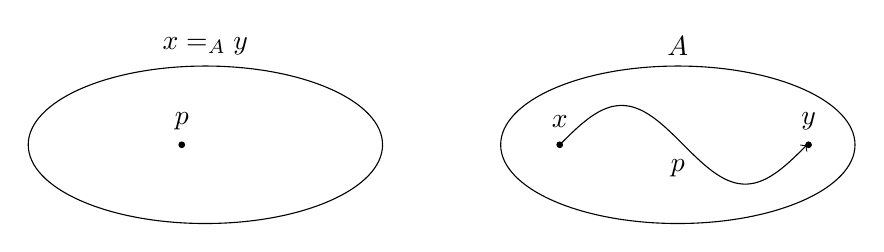
\begin{tikzpicture}
        \tikzstyle{every node}=[font=\normalsize]
        \draw(0.5,0) ellipse (2.25cm and 1cm);
        \draw(6.5,0) ellipse (2.25cm and 1cm);
        \node[font=\normalsize] at (6.5,1.25) {$A$};
        \node[font=\normalsize] at (0.5,1.25) {$x =_A y$};
    
         % Draw the sine wave
        \draw[->,domain=0:3.14,smooth,variable=\x] plot ({\x + 5},{0.5*sin(2*\x r)});
     
        \filldraw(0.2,0) circle (1pt);
        \filldraw(5,0) circle (1pt);
        \filldraw(8.16,0) circle (1pt);

        \node[font=\normalsize] at (0.2,0.3) {$p$};
        \node[font=\normalsize] at (5,0.3) {$x$};
        \node[font=\normalsize] at (8.16,0.3) {$y$};
        \node[font=\normalsize] at (6.5,-0.3) {$p$};
    \end{tikzpicture}
    \label{fig:id_type}
    \caption{Геометријска репрезентација типова идентитета. Лело је представљена класична интерпретација, у којој $x =_A y$ представља исказ, са много различитих сведока $p : x =_A y$ који оправдавају његову истинитост. Док је десно представљена хомотопна интерпретација, у којој између тачака $x$ и $y$ постоји много различитих путања $p$ у простору $A$.}
\end{figure}

Ако је $A$ тип и ако су дати елементи $x, y : A$ у контексту $\Gamma$, онда можемо формирати тип идентитета $x =_A y$ кога ће настањивати путање, еквиваленције или идентификације. Основна идентификација коју можемо да конструишемо је \emph{рефлексија}:
\[ \refl{x} : x =_A x. \]
Рефлексија $\refl{x}$ тврди да је било који елемент $x : A$ једнак самом себи. Рефлексију $\refl{x}$, у хомотопном смислу, можемо посматрати као константну путању у тачки $x : A$. Формално, начин формирања и конструисања типова идентитета дат је следећом спецификацијом:

\begin{samepage}
    \begin{center}
        \begin{minipage}{0.49\textwidth}
            \begin{prooftree}[$=$-form]
                \AxiomC{$\Gamma \vdash A~\type$}
                \AxiomC{$\Gamma \vdash x : A$}
                \AxiomC{$\Gamma \vdash y : A$}
                \TrinaryInfC{$\Gamma \vdash x=_{A}y~\type$}
            \end{prooftree}
        \end{minipage}
        \begin{minipage}{0.39\textwidth}
            \begin{prooftree}[$=$-intro]
                \AxiomC{$\Gamma \vdash A~\type$}
                \AxiomC{$\Gamma \vdash x : A$}
                \BinaryInfC{$\Gamma \vdash \refl{x} : x=_{A}x$}
            \end{prooftree}
        \end{minipage}
    \end{center}
\end{samepage}

Уколико су два елемента $x, y : A$ расуђивачки једнака, тј. важи $x \equiv_A y$, онда су и исказно једнака и важи $\refl{x} : x =_A y$. Оправдање проналазимо у $\refl{x} : (x =_A x) \equiv (x =_A y)$, јер важи $x \equiv_A y$. Обратно, у општем сличају, не важи. Другим речима, уколико су два елемента $x, y : A$ исказно једнака, тј. важи $x =_A y$, у општем случају, неће бити расуђивачки једнака, тј. не важи $x \equiv_A y$. Због тога, расуђивачку једнакост често можемо посматрати као \emph{дефинициону једнакост}.

\subsection{Индукција путање}

Правило индукције за типове идентитета називамо \emph{индукција путање}. Индукција путање тврди да за било коју фамилију типова $P$ над типовима $A$ и $x =_A y$ постоји функција $\ind{=} : \prod_{(x, y : A)} \prod_{(p : x =_{A} y)} P(x, y, p)$ уколико постоји функција $f : \prod_{(x : A)} P(x, x, \refl{x})$. Како постоји само један конструктор $\refl{x} : x =_A x$, постоји само једно правило израчунавања које треба да се поклопи са правилом индукције. Због тога је правило израчунавања $\ind{=}(x, x, \refl{x}) \equiv f(x) : P(x, x, \refl{x})$. Формално, правило индукције и правило израчунавања је дато следећом спецификацијом:

\begin{samepage}
    \begin{center}
        \begin{minipage}{\textwidth}
            \begin{prooftree}[$=$-ind]
                \def\fCenter{\Gamma}
                \Axiom$\fCenter, x : A, y : A, p : x =_{A} y \vdash P(x, y, p)~\type$
                \noLine%
                \UnaryInf$\fCenter\ \vdash f : \prod_{(x : A)} P(x, x, \refl{x})$
                \UnaryInf$\fCenter\ \vdash \ind{=} : \prod_{(x, y : A)} \prod_{(p : x =_{A} y)} P(x, y, p)$
            \end{prooftree}
        \end{minipage}
        \begin{minipage}{\textwidth}
            \begin{prooftree}[$=$-comp]
                \def\fCenter{\Gamma}
                \Axiom$\fCenter, x : A, y : A, p : x =_{A} y \vdash P(x, y, p)~\type$
                \noLine%
                \UnaryInf$\fCenter\ \vdash f : \prod_{(x : A)} P(x, x, \refl{x})$
                \UnaryInf$\fCenter, x : A \vdash \ind{=} (x, x, \refl{x}) \equiv f(x) : P(x, x, \refl{x})$
            \end{prooftree}
        \end{minipage}
    \end{center}
\end{samepage}

Једно од кључних питања је шта оправдава индукцију путањом? Другим речима, зашто ће $P(x, y, p)$ важити за било које тачке $x, y : A$ и било коју путању $p: x =_A y$ уколико важи $P(x, x, \refl{x})$ за било коју тачку $x : A$? Кључно запажање лежи у томе да типови идентитета нису индуктивни тип, већ да су индуктивна фамилија типова. То значи да индукција путањом тврди да је фамилија типова $x =_A y$, где су $x$ и $y$ слободне тачке простора $A$, индуктивно дефинисана константном путањом
$\refl{x}$. Односно, $\sum_{(x, y : A)} (x =_A y)$ је индуктивно генерисан константним путањама у свакој такчи $x : A$. Битно је напоменути да су обе тачке слободне. Такође, можемо фиксирати једну тачку (у том случају долазимо до другачије еквивалентне индукције путањом, која се назива и \emph{базна индукција путањом}).  

\begin{figure}[!ht]
    \centering\
    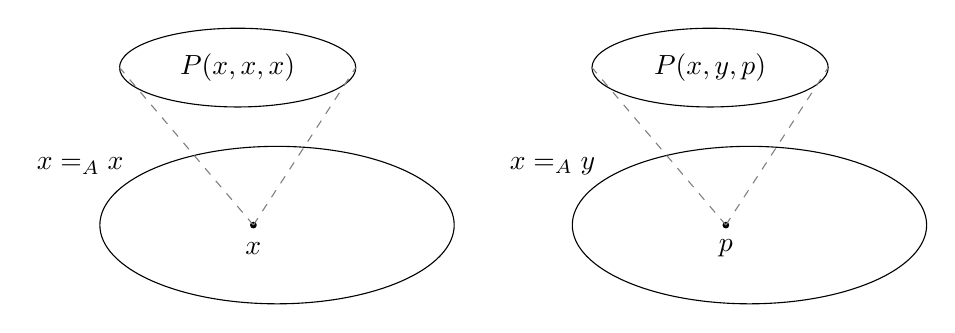
\begin{tikzpicture}
        \tikzstyle{every node}=[font=\normalsize]
        \draw(0.5,0) ellipse (2.25cm and 1cm);
        \draw(6.5,0) ellipse (2.25cm and 1cm);
        \node[font=\normalsize] at (4,0.75) {$x =_A y$};
        \node[font=\normalsize] at (-2,0.75) {$x =_A x$};
    
        \draw(0,2) ellipse (1.5cm and 0.5cm);
        \draw(6,2) ellipse (1.5cm and 0.5cm);
     
        \filldraw(0.2,0) circle (1pt);
        \filldraw(6.2,0) circle (1pt);
 

        \node[font=\normalsize] at (0.2,-0.3) {$\refl{x}$};
        \node[font=\normalsize] at (6.2,-0.3) {$p$};

        \draw[color=gray, dashed] (0.2,0)-- (-1.5,2);
        \draw[color=gray, dashed] (0.2,0)-- (1.5,2);
        \draw[color=gray, dashed] (6.2,0)-- (4.5,2);
        \draw[color=gray, dashed] (6.2,0)-- (7.5,2);

        \node[font=\normalsize] at (0,2) {$P(x, x, \refl{x})$};
        \node[font=\normalsize] at (6,2) {$P(x, y, p)$};

    \end{tikzpicture}
    \label{fig:path_ind}
    \caption{Геометријска репрезентација индукције путањом.}
\end{figure}

Неформално, оправдање индукција путањом је осликано следећим примером: Посматрајмо петљу на пробушениом диску која полази из једне тачке, обилази једном рупу, и враћа се у исту тачку. Уколико су почетна тачка и крајња тачка фиксиране, није могуће непрекидно деформисати петљу у константну путању. Када допустимо један крај петље да буде слободна, он може обићи рупу, те је могуће непрекидно деформисати петљу у константну путању. Слично је могуће ако допустимо да обе краја петље буду слободна. 

\subsection{Особине типова идентитета}

У хомотопној теорији, над тополошким простором $A$, \emph{путања} између две тачке $x$ и $y$ представља непрекидно пресликавање $p : [0, 1] \to A$, за које важи $p(0) = x$ и $p(1) = y$. Путања $p : [0, 1] \to A$ је \emph{петља} уколико почиње и завршава се у тачки $a_0$, тј. важи $a_0 = p(0) = p(1)$. Једни од корисних појмова над путањама су инверз путање и надовезивање путања. \emph{Инверз путање} $p : [0, 1] \to A$ је путања $p^{-1} : [0, 1] \to A$ за коју важи $p^{-1} (t) = p (1 - t)$ за свако $t \in [0, 1]$. \emph{Надовезивање путања} $p : [0, 1] \to A$ и $q : [0, 1] \to A$ којима се крај и почетак поклапају, тј. за које $p(1) = q(0)$, представља путању $p \cdot q : [0, 1] \to A$ за коју важи $(p \cdot q) (t) = p(2t)$ за свако $t \in [0, 1/2]$, и $(p \cdot q) (t) = q(2t - 1)$ за свако $t \in [1/2, 1]$. Инверз путање и надовезивање путања, у теорији типова, се карактеришу преко типова идентитета и дате су у следећим лемама:

\begin{lemma}
    Нека је $A$ тип у контексту $\Gamma$. Тада можемо конструисати функцију \[\inv{A} : \prod_{(x, y : A)} (x =_A y) \to (y =_A x)\] индукцијом путање $p : x =_A y$ као $\inv{A} (x, x, \refl{x}) :\equiv \refl{x}$. Функцију $\inv{A}$ називамо \emph{инверз путање}. Често, за дату путању $p : x =_A y$, њен инверз означавамо са $p^{-1} :\equiv \inv{A}(x, y, p)$.
\end{lemma}
\begin{proof}
    Да би констурисали елемент типа $\prod_{(x,y : A)} (x =_A y) \to (y =_A x)$, конструишемо функцију \[ f(x) : \prod_{(y : A)} (x =_A y) \to (y =_A x)\] за било који елемент $x : A$. По индукцији путање $p : x =_A y$ довољно је конструисати путању \[ f(x, x, \refl{x}) : x =_A x \] за било који елемент $x : A$. Конструкција ове путање је тривијална и због тога узимамо да је $f (x, x, \refl{x}) :\equiv \refl{x}$. Коначно, тражена конструкција је \[ \inv{A} (x, x, \refl{x}) :\equiv \refl{x}. \] 
\end{proof}

\begin{lemma}
    Нека је $A$ тип у контексту $\Gamma$. Тада можемо конструисати функцију \[\conc{A} : \prod_{(x, y, z : A)} (x =_A y) \to (y =_A z) \to (x =_A z)\] индукцијом путање $p : x =_A y$ као $\conc{A} (x, x, z, \refl{x}, q) :\equiv q$. Функцију $\conc{A}$ називамо \emph{надовезивање путања}. Често, за дате путање $p : x =_A y$ и $q : y =_A z$, надовезану путању означавамо са $p \cdot q :\equiv \conc{A} (x, y, z, p, q)$.
\end{lemma}
\begin{proof}
    Прво конструишемо функцију
    \[f(x) : \prod_{(y : A)} (x =_A y) \to \prod_{(z : A)} (y =_A z) \to (x =_A z)\] за било који елемент $x : A$. По индукцији путање $p : (x =_A y)$ довољно је конструисати функцију \[ f(x, x, \refl{x}) : \prod_{(z : A)} (x =_A z) \to (x =_A z) \] за било који елемент $x : A$. Даље, довољно је конструисати функцију \[ f(x, x, \refl{x}, z) : (x =_A z) \to (x =_A z) \] за било које елементе $x, z : A$. Конструисање ове функције је тривијално и због тога имамо да је $f(x, x, \refl{x}, z, q) :\equiv q$. Коначно, тражена конструкција је \[\conc{A}(x, x, z, \refl{x}, q) :\equiv f(x, x, \refl{x}, z, q) :\equiv q. \]
\end{proof}

Код једнакосне логике, инверз путање представља особину симетрије једнакости, док надовезивање путања представља особину транзитивности једнакости. Транзитивност једнакости се користи када доказујемо неку једнакости ланцем једнакости. На пример, уколико желимо да пронађемо сведока за $a = d$, и знамо да су $p : a = b$, $q : b = c$ и $r : c = d$, једноставним надовезивањем путања добијамо сведока $(p \cdot q) \cdot r : a = d$. Ово може бити тешко за тумачење па се често користи следећа синтакса:
\begin{align*}
    a &= b & (p) \\
      &= c & (q) \\
      &= d & (r).
\end{align*}

Строге једнакости над путањама често нису корисне. Због тога, дефинишемо појам хомотопије. \emph{Хомотопија} између две путање $p : [0, 1] \to A$ и $q : [0, 1] \to A$ је непрекидно пресликавање $H : [0, 1] \times [0, 1] \to A$, за које важи $H(s, 0) = p(s)$ и $H(s, 1) = q(s)$ за свако $s \in [0, 1]$, и
$H(0, t) = x$ и $H(1, t) = y$ за свако $t \in [0, 1]$. За две путање кажемо да су \emph{хомотопне}, уколико постоји хомотопија између њих.

Релација хомотопности између две путање је релација еквиваленције, и операције инверз путање и надовезивање путања одржавају еквиваленцију. Над простором $A$, класа еквиваленција хомотопних петљи у тачки $a_0$ формира групу коју називамо \emph{фундаментална група} и обележавамо са $\pi_1(A, a_0)$. За разлику од простора свих петљи у тачки $a_0$, фундаментална група $\pi_1(A, a_0)$ нам омогућава да лакше испитујемо простор $A$. Прецизније, фундаментална група је алгебарска инваријанта
простора, која може да се искористи за испитивање \emph{хомотопне еквиваленције} два простора.

Хомотопију можемо сматрати као дводимензиону путању, то природно можемо уопштити на тродимензиону путању, четвородимензиону путању, итд. Ово нам дају бесконачни низ појмова: тачка, путања, хомотопија, хомотопија између хомотопија, хомотопија између хомотопија између хомотопија, итд. Заједно са операцијама фундаменталне групе (константна путања, инверз путање, надовезивање путања) добијамо инстанцу алгебарске структуре која се зове (\emph{слаби}) $\infty$-\emph{групоид}.

$\infty$-групоид представља алгебарску структуру која садржи колекцију \emph{објеката} и колекцију \emph{морфизама} између објеката, \emph{морфизама између морфизама}, итд. Морфизме на ниву $k$ зовемо $k$-морфизми. Морфизми сваког нивоа имају комплексну алгебарску структуру, па тако у случају слабог $\infty$-групоида, сваки морфизам датог нивоа има идентитет, композицију, и инверз који задовољавају закон асоцијативности, идентитета и инверза, до на морфизме следећег нивоа.

Ову идеју можемо интерпретирати у теорији типова преко типова идентитета. На основном нивоу имамо елементе неког типа које можемо да идентификујемо. На пример, за $x, y : A$, разматрамо идентификацију $x =_A y$. Како је теорија типова доказно релевантна, могуће је да постоји више различитих сведока за $x =_A y$. Нека су то путање $p, q : x =_A y$. Типови идентитета нам даље омогућавају да разматрамо једнакост између $p$ и $q$, односно омогућавају нам да формирамо тип $p =_{x =_A y} q$. Како су $p$ и $q$ путање, сведока $r : p =_{x =_A y} q$ можемо сматрати као хомотопијом између путања $p$ и $q$, или као дводимензионом путањом. Можемо даље итерирати и добити тип тродимензионих путања $r =_{p =_{x =_A y} q} s$, итд. У табели~\ref{table:inftygroupoid} приказана је веза између једнакосне логике, хомотопне теорија и структуре $\infty$-групоид.

\begin{table}
    \begin{center}
        \begin{tabular}[c]{l l l}
            Једнакости & Хомотопија & $\infty$-Групоид \\
            \hline%
            рефлексивност & константна путања & идентички морфизам \\
            симетричност & обртање путања & инверз морфизма \\
            транзитивност & надовезивање путања & компоизиција морфизама\\
        \end{tabular}
    \end{center}
    \caption{Разне интерпретације особина типова идентитета}
    \label{table:inftygroupoid}
\end{table}

На слици~\ref{fig:inftygroupoid} приказана је групоидална структура типова, док следећа лема карактерише да тип идентитета на датом нивоу има својства слабог $\infty$-групоида:

\begin{lemma}
    Нека је $A$ тип, нека су елементи $x, y, z, w : A$ и нека су путање $p : x =_A y,\, q : y =_A z$ и $r : z =_A w$ у контексту $\Gamma$. Тада важи:
    \begin{enumerate}[(i)]
        \item $\refl{x} \cdot p = p$ и $p \cdot \refl{y} = p$
        \item $p^{-1} \cdot p = \refl{y}$ и $p \cdot p^{-1} = \refl{x}$
        \item $(p^{-1})^{-1} = p$
        \item $(p \cdot q) \cdot r = p \cdot (q \cdot r)$
    \end{enumerate}
\end{lemma}
\begin{enumerate}[(i)]
    \item 
    \begin{proof}
        Желимо да конструишемо путању
        \begin{align*}
            \mathsf{unit_l}(p) &: \refl{x} \cdot p = p, \\
            \mathsf{unit_r}(p) &: p \cdot \refl{y} = p. \\
        \end{align*} 
        Индукцијом по путањи $p : x =_A y$ довољно је конструисати
        \begin{align*}
            \mathsf{unit_l}(\refl{x}) &: \refl{x} \cdot \refl{x} = \refl{x}, \\
            \mathsf{unit_r}(\refl{x}) &: \refl{x} \cdot \refl{x} = \refl{x}.
        \end{align*} 
        Обе путање је тривијално конструисати као $\refl{\refl{x}}$.
    \end{proof}
    \item 
    \begin{proof}
        Желимо да конструишемо путању
        \begin{align*}
            \mathsf{inv_l}(p) &: p^{-1} \cdot p = \refl{y}, \\
            \mathsf{inv_r}(p) &: p \cdot p^{-1} = \refl{x}.
        \end{align*}
        Индукцијом по путањи $p : x =_A y$ довољно је конструисати путању
        \begin{align*}
            \mathsf{inv_l}(\refl{x}) &: \refl{x}^{-1} \cdot \refl{x} = \refl{x}, \\
            \mathsf{inv_r}(\refl{x}) &: \refl{x} \cdot \refl{x}^{-1} = \refl{x}.
        \end{align*}
        Али како је $\refl{x}^{-1} \equiv \refl{x}$ претходне путање се своде на оне као и у претходном доказу. Због тога обе путање тривијално конструишемо као $\refl{\refl{x}}$.
    \end{proof}
    \item
    \begin{proof}
        Желимо да конструишемо путању
        \[ \mathsf{doubleInv} (p) : (p^{-1})^{-1} = p. \]
        Индукцијом по путањи $p : x =_A y$ довољно је конструисати путању
        \[ \mathsf{doubleInv} (\refl{x}) : (\refl{x}^{-1})^{-1} = \refl{x}. \]
        Али како је $(\refl{x}^{-1})^{-1} \equiv \refl{x}^{-1} \equiv \refl{x}$ претходна путања се своди на $\refl{x} = \refl{x}$. Због тога путању тривијално конструишемо као $\refl{\refl{x}}$. 
    \end{proof} 
    \item
    \begin{proof}
        Желимо да конструишемо путању
        \[ \assoc{A} (p, q, r) : (p \cdot q) \cdot r = p \cdot (q \cdot r). \]
        Индукцијом по путањи $p : x =_A y$ довољно је конструисати путању
        \[ \assoc{A} (\refl{x}, q, r) : (\refl{x} \cdot q) \cdot r = \refl{x} \cdot (q \cdot r) \]
        Али како је $\refl{x} \cdot q \equiv q$ и $\refl{x} \cdot (q \cdot r) \equiv q \cdot r$ претходна путања се своди на
        \[ \assoc{A} (\refl{x}, q, r) : q \cdot r = q \cdot r. \]
        Због тога путању тривијално конструишемо као $\assoc{A} (\refl{x}, q, r) :\equiv \refl{q \cdot r}$.
    \end{proof}
\end{enumerate}

\begin{figure}[!ht]
    \centering\
    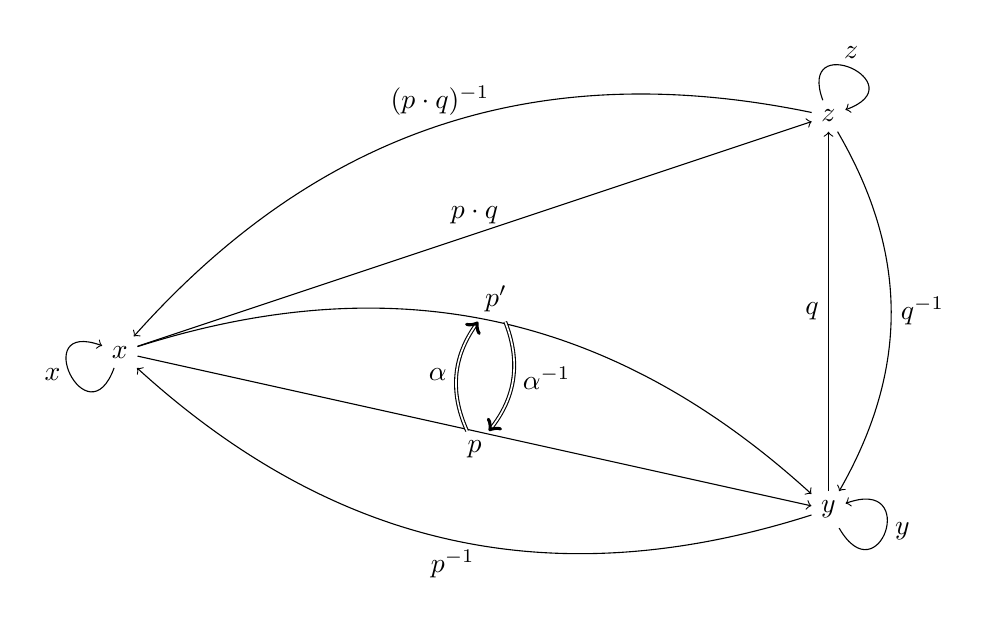
\begin{tikzpicture}
        \tikzstyle{every node}=[font=\normalsize]
        \node (X) at (0,2) {$x$};
        \node (Y) at (9,0) {$y$};
        \node (Z) at (9,5) {$z$};
        \draw[->] (X) -- (Y) node[midway, below] (P) {$p$};
        \draw[->] (Y) -- (Z) node[midway, left] {$q$};
        \draw[->] (X) -- (Z) node[midway, above] {$p \cdot q$};
        \draw[<-] (X) to[bend right] node[midway, below] {$p^{-1}$} (Y);
        \draw[->] (X) to[bend left] node[midway, above] (P') {$p'$} (Y);
        \draw[<-] (Y) to[bend right] node[midway, right]  {$q^{-1}$} (Z);
        \draw[<-] (X) to[bend left] node[midway, above] (PQ) {$(p \cdot q)^{-1}$} (Z);
        \draw[->, double] (P) to[bend left] node[midway, left] {$\alpha$} (P');
        \draw[<-, double] (P) to[bend right] node[midway, right] {$\alpha^{-1}$} (P');
        \draw[->, loop above] (X) to[out=250, in=160, looseness=8] node[left] {$\refl{x}$} (X);
        \draw[->, loop above] (Y) to[out=300, in=380, looseness=8] node[right] {$\refl{y}$} (Y);
        \draw[->, loop above] (Z) to[out=110, in=20, looseness=8] node[above] {$\refl{z}$} (Z);
    \end{tikzpicture}
    \label{fig:inftygroupoid}
    \caption{Групоидална структура типова. }
\end{figure}

\subsection{Акције над путањама}

Функција $f : A \to B$ се понаша као функтор у односу на путање. Другим речима, функције поштују једнакости, или функције одржавају путање. Ова особина дата је следећом лемом:

\begin{lemma}
    Нека су $A$ и $B$ типови, и нека је $f : A \to B$ функција у контексту $\Gamma$. Тада можемо конструисати функцију 
    \[\ap{f} : \prod_{(x,y:A)} (x =_{A} y) \to (f (x) =_{B} f (y))\]
    индукцијом путање $p : x =_{A} y$ као $\ap{f} (\refl{x}) = \refl{f(x)}$. Функцију $\ap{f}$ називамо \emph{акција над путањамa} функције $f : A \to B$.
\end{lemma}
\begin{proof}
    Индукцијом по путањи $p : x =_{A} y$ треба конструисати путању
    \[\ap{f} (x, x, \refl{x}) : f(x) =_B f(x).\]
    Тривијално конструишемо ову путању као $\ap{f} (x, x, \refl{x}) :\equiv \refl{f(x)}$.
\end{proof}

Важе уобичајене особине за функторе:

\begin{lemma}
    Нека су $A, B$ и $C$ типови, нека су елементи $x, y, z : A$ и нека су путање $p : x =_A y$ и $q : y =_A z$ у контексту $\Gamma$. Тада важи:
    \begin{enumerate}[(i)]
        \item $\ap{f} (p \cdot q) = \ap{f}(p) \cdot \ap{f}(q)$
        \item $\ap{f} (p^{-1}) = \ap{f}(p)^{-1}$
        \item $\ap{g} (\ap{f} (p)) = \ap{g \circ f} (p)$
        \item $\ap{\id{A}} (p) = p$
    \end{enumerate}
\end{lemma}
\begin{proof}
    Доказ изостављамо како је сличан претходним.
\end{proof}

\subsection{Транспорт}

Уколико посматрамо функцију $f : \prod_{(x : A)} B(x)$ и путању $p : x =_A y$, онда не можемо размазрати једнакост елемената $f(x) : B(x)$ и $f(y) : B(y)$, јер нису истог типа. Али можемо разматрати функцију $B(x) \to B(y)$, коју карактерише следећа лема:

\begin{lemma}
    Нека је $A$ тип и $B$ фамилија типова над $A$ у контексту $\Gamma$. Тада можемо конструисати функцију
    \[\tr{B} : \prod_{(x,y:A)} (x =_{A} y) \to B(x) \to B(y)\]
    индукцијом путање $p : x =_{A} y$ као $\tr{B}(\refl{x}) :\equiv \mathsf{id}_{B(x)}$.
Функцију $\tr{B}$ називамо \emph{транспорт} над $B$.
\end{lemma}
\begin{proof}
    Индукцијом по путањи $p : x =_{A} y$ треба конструисати функцију
    \[\tr{B}(x, x, \refl{x}) \to B(x) \to B(x).\]
    Тривијално конструишемо ову путању као $\tr{B} (x, x, \refl{x}) :\equiv \id{B(x)}$.
\end{proof}

Фамилија типова $B$ над типом $A$, може се сматрати као својство елемената типа $A$. Другим речима, $B(x)$ је својство елемента $x : A$. Због тога и претходне леме, можемо тврдити да својства поштују једнакости, у смислу да ако је $x =_A y$, онда $B(x)$ акко $B(y)$.

\subsection{Друге врсте једнакости}

Некада расуђивачка и исказна једнакост нису довољне да би се показале све тврдње. На пример, не можемо пронаћи сведоке за $\neg (\succN(n) =_\N \zeroN)$ и $(\succN(m) =_\N \succN(n)) \to m =_\N n$ без следеће карактеризације:

\begin{definition}
    \label{def:code}
    \emph{Простор кодова} над природним бројевима $\N$ се може дефинисати као бинарна релација $\codee{\N} : \N \to \N \to \mathcal{U}_0$ тако да задовољава следеће расуђивачке једнакости:
    \begin{align*}
        \codee{\N} (\zeroN, \zeroN) &\equiv\1 \\
        \codee{\N} (\zeroN, \succN(m)) &\equiv\0 \\
        \codee{\N} (\succN(n), \zeroN) &\equiv\0 \\
        \codee{\N} (\succN(n), \succN(m)) &\equiv\codee{\N} (n, m) \\
    \end{align*}
\end{definition}

\begin{lemma}
    Простор кодова је рефлексивна релација, тј.~можемо конструисати функцију
    \[\refl{}\codee{\N} : \prod_{(n : \N)} \codee{\N} (n, n).\]
\end{lemma}
\begin{proof}
    Функцију конструишемо индукцијом по $n : \N$ као
    \begin{align*}
        \refl{}\codee{\N} (\zeroN) &:\equiv \star \\
        \refl{}\codee{\N} (\succN(n)) &:\equiv \refl{}\codee{\N} (n).
    \end{align*}
\end{proof}

\begin{lemma}
    За било које природне бројеве $n, m : \N$ важи $m =_{\N} n \to \codee{\N} (m, n)$ и $\codee{\N} (m, n) \to m =_{\N} n$.
\end{lemma}
\begin{proof}
    Прво конструишемо
    \[ \encode{\N} : \prod_{(m, n : \N)} m =_{\N} n \to \codee{\N}(m, n). \]
    Индукцијом по путањи $p : m =_{\N} n$ треба конструисати 
    \[ \encode{\N} (m, m, \refl{m}) : \codee{\N} (m, m). \]
    Што смо конструисали у претходној леми, тако да $\encode{\N} (m, m, \refl{m}) :\equiv \refl{}\codee{\N} (m)$.
    Даље конструишемо
    \[ \decode{\N} : \prod_{(m, n : \N)} \codee{\N}(m, n) \to m =_{\N} n \]
    индукцијом по $m : \N$ и $n : \N$. У случају када су оба природна броја нуле, онда $\decode{\N} (\zeroN, \zeroN, c) : \zeroN =_{\N} \zeroN$ конструишемо као $\decode{\N} (\zeroN, \zeroN, c) :\equiv \refl{\zeroN}$.
    У случају када је тачно један од њих нула, тада конструишемо елемент типа $\0 \to m =_{\N} n$. Овај елемент је тривијално конструисати правилом индукције празног типа. На крају, у случају када су оба различита од нуле, треба конструисати  
    \[ \codee{\N} (\succN(m), \succN(n)) \to \succN(m) =_{\N} \succN(n). \]
    Ову конструкцију изводимо на следећи начин:
    \begin{align*}
        \codee{\N} (\succN(m), \succN(n)) &\equiv \codee{\N} (m, n) &\quad (\text{деф. }\ref{def:code})\\
                                         &\to  m =_{\N} n &\quad (\decode{\N}(m, n)) \\
                                         &\to \succN(m) =_{\N} \succN(n) &\quad (\ap{\succN}).
    \end{align*}
    Коначно, завршавамо конструкцију са 
    \[ \decode{\N}(\succN(m), \succN(n), c) :\equiv \ap{\succN} (\decode{\N}(m, n, c)). \]
\end{proof}

% ------------------------------------------------------------------------------
\chapter{\textsc{Agda}}
% ------------------------------------------------------------------------------

\textsc{Agda} је типски завистан програмски језик који проширује МЛТТ. Језик \textsc{Agda} подсећа на функционалне програмске језике као што је \textsc{Haskell}, али их проширује зависним типовима. Са друге стране, \textsc{Agda} је интерактивни доказивач теорема. Њена предност у односу на друге интерактивне доказиваче, је минималност, и високи степен модуларности и изражајности. То је чини идеалним интерактивним доказивачем за формализовање МЛТТ-a, па самим тим и ХоТТ-a.  

\section{Упутство за коришћење језика \textsc{Agda}}
Прођимо кроз један основни пример формализације типа природних бројева. Како се име сваког \textsc{Agda} фајла завршава екстензијом \texttt{.agda}, нека се наш фајл зове \texttt{Tutorial.agda}.

На почетку фајла описујемо неке мета-податке:
\begin{code}%
\>[0]\AgdaSymbol{\{-\#}\AgdaSpace{}%
\AgdaKeyword{OPTIONS}\AgdaSpace{}%
\AgdaPragma{--without-K}\AgdaSpace{}%
\AgdaPragma{--safe}\AgdaSpace{}%
\AgdaSymbol{\#-\}}\<%
\end{code}
У овом случају то су опције \texttt{--without-K} и \texttt{--safe}, које обезбеђују рад на ХоТТ-у. Више детаља се може наћи на званичној документацији језика \textsc{Agda}~\cite{agda_manual}.

\textsc{Agda} програм је сачињен од \emph{модула}. Сваки модул има своје име (које мора да се поклопи са именом фајла) као и низ декларација. Модул за наш фајл \texttt{Tutorial.agda} започињемо на следећи начин:
\begin{code}%
\>[0]\AgdaKeyword{module}\AgdaSpace{}%
\AgdaModule{Tutorial}\AgdaSpace{}%
\AgdaKeyword{where}\<%
\end{code}

Једна врста декларација је увожење других модула. Тако, на пример, можемо увести модул \texttt{Universes} на следећи начин: 
\begin{code}%
\>[0]\AgdaKeyword{open}\AgdaSpace{}%
\AgdaKeyword{import}\AgdaSpace{}%
\AgdaModule{Universes}\AgdaSpace{}%
\AgdaKeyword{public}\<%
\end{code}

Друга врста декларација је декларисање променљивих. На пример, можемо рећи да $\mathcal{U}$, $\mathcal{V}$ и $\mathcal{W}$ представљају универзум:
\begin{code}%
\>[0]\AgdaKeyword{variable}\AgdaSpace{}%
\AgdaGeneralizable{𝓤}\AgdaSpace{}%
\AgdaGeneralizable{𝓥}\AgdaSpace{}%
\AgdaGeneralizable{𝓦}\AgdaSpace{}%
\AgdaSymbol{:}\AgdaSpace{}%
\AgdaPostulate{Universe}\<%
\end{code}

Једна од кључних декларација је декларација индуктивних типова. Декларисање индуктивних типова подразумева навођење имена тог типа, начин на који се он формира, као и начин за конструисање каноничних елемената тог типа. У теорији типова, то смо називали правило формирања типова и правила конструисања (за детаље видети поглавље~\ref{sec:indtyp}). Подсетимо се правила формирања и правила конструисања типа природних бројева $\N$. Тип природних бројева $\N$ може да се формира из празног контекста, односно $\N : \mathcal{U}_0$, као и да су му једини конструктори $\zeroN : \N$ и $\succN : \N \to \N$. У језику \textsc{Agda} то записујемо као: 
\begin{code}%
\>[0]\AgdaKeyword{data}\AgdaSpace{}%
\AgdaDatatype{ℕ}\AgdaSpace{}%
\AgdaSymbol{:}\AgdaSpace{}%
\AgdaPrimitive{𝓤₀}\AgdaSpace{}%
\AgdaOperator{\AgdaFunction{̇}}\AgdaSpace{}%
\AgdaKeyword{where}\<%
\\
\>[0][@{}l@{\AgdaIndent{0}}]%
\>[4]\AgdaInductiveConstructor{zero}\AgdaSpace{}%
\AgdaSymbol{:}\AgdaSpace{}%
\AgdaDatatype{ℕ}\<%
\\
%
\>[4]\AgdaInductiveConstructor{succ}\AgdaSpace{}%
\AgdaSymbol{:}\AgdaSpace{}%
\AgdaDatatype{ℕ}\AgdaSpace{}%
\AgdaSymbol{→}\AgdaSpace{}%
\AgdaDatatype{ℕ}\<%
\\
\>[0]\<%
\\
\>[0]\AgdaSymbol{\{-\#}\AgdaSpace{}%
\AgdaKeyword{BUILTIN}\AgdaSpace{}%
\AgdaKeyword{NATURAL}\AgdaSpace{}%
\AgdaDatatype{ℕ}\AgdaSpace{}%
\AgdaSymbol{\#-\}}\<%
\end{code}
Опција \texttt{BUILTIN NATURAL} $\N$ обезбеђује да каноничне елементе типа природних бројева $\zeroN, \succN(\zeroN), \succN(\succN(\zeroN)), \ldots$ можемо да записујемо као $0, 1, 2, \ldots$. 

Поред правила формирања и правила конструисања, за комплетну спецификацију индуктивних типова имали смо и правило индукције и правило израчунавања (за детаље видети поглавље~\ref{sec:indtyp}). Правило индукције типа природних бројева $\N$, у језику \textsc{Agda} записујемо као:
\begin{code} %
\>[0]\AgdaFunction{ℕ-induction}%
\>[29I]\AgdaSymbol{:}\AgdaSpace{}%
\AgdaSymbol{(}\AgdaBound{P}\AgdaSpace{}%
\AgdaSymbol{:}\AgdaSpace{}%
\AgdaDatatype{ℕ}\AgdaSpace{}%
\AgdaSymbol{→}\AgdaSpace{}%
\AgdaPrimitive{𝓤₀}\AgdaSpace{}%
\AgdaOperator{\AgdaFunction{̇}}\AgdaSpace{}%
\AgdaSymbol{)}\<%
\\
\>[.][@{}l@{}]\<[29I]%
\>[12]\AgdaSymbol{→}\AgdaSpace{}%
\AgdaBound{P}\AgdaSpace{}%
\AgdaNumber{0}\<%
\\
%
\>[12]\AgdaSymbol{→}\AgdaSpace{}%
\AgdaSymbol{((}\AgdaBound{n}\AgdaSpace{}%
\AgdaSymbol{:}\AgdaSpace{}%
\AgdaDatatype{ℕ}\AgdaSymbol{)}\AgdaSpace{}%
\AgdaSymbol{→}\AgdaSpace{}%
\AgdaBound{P}\AgdaSpace{}%
\AgdaBound{n}\AgdaSpace{}%
\AgdaSymbol{→}\AgdaSpace{}%
\AgdaBound{P}\AgdaSpace{}%
\AgdaSymbol{(}\AgdaInductiveConstructor{succ}\AgdaSpace{}%
\AgdaBound{n}\AgdaSymbol{))}\<%
\\
%
\>[12]\AgdaSymbol{→}\AgdaSpace{}%
\AgdaSymbol{(}\AgdaBound{n}\AgdaSpace{}%
\AgdaSymbol{:}\AgdaSpace{}%
\AgdaDatatype{ℕ}\AgdaSymbol{)}\AgdaSpace{}%
\AgdaSymbol{→}\AgdaSpace{}%
\AgdaBound{P}\AgdaSpace{}%
\AgdaBound{n}\<%
\end{code}
Приметимо да у формулацији правила индукције фамилију типова $P$ над типом природних бројева $\N$ записујемо као $P : \N \to \mathcal{U}_0$, као и да зависну функцију $\prod_{(n : \N)} P (n)$ записујемо као $(n : \N) \to P~n$.

Са друге стране, правила израчунавања записујемо као:
\begin{code}%
\>[0]\AgdaFunction{ℕ-induction}\AgdaSpace{}%
\AgdaBound{P}\AgdaSpace{}%
\AgdaBound{p₀}\AgdaSpace{}%
\AgdaBound{pₛ}\AgdaSpace{}%
\AgdaInductiveConstructor{zero}%
\>[29]\AgdaSymbol{=}\AgdaSpace{}%
\AgdaBound{p₀}\<%
\\
\>[0]\AgdaFunction{ℕ-induction}\AgdaSpace{}%
\AgdaBound{P}\AgdaSpace{}%
\AgdaBound{p₀}\AgdaSpace{}%
\AgdaBound{pₛ}\AgdaSpace{}%
\AgdaSymbol{(}\AgdaInductiveConstructor{succ}\AgdaSpace{}%
\AgdaBound{n}\AgdaSymbol{)}\AgdaSpace{}%
\AgdaSymbol{=}\AgdaSpace{}%
\AgdaBound{pₛ}\AgdaSpace{}%
\AgdaBound{n}\AgdaSpace{}%
\AgdaSymbol{(}\AgdaFunction{ℕ-induction}\AgdaSpace{}%
\AgdaBound{P}\AgdaSpace{}%
\AgdaBound{p₀}\AgdaSpace{}%
\AgdaBound{pₛ}\AgdaSpace{}%
\AgdaBound{n}\AgdaSymbol{)}\<%
\end{code}

У многим случајевима \textsc{Agda} може помоћи при декларисању правила израчунавања. Како она описују начин конструисања елемента који оправдава правило индукције можемо поћи од:
\begin{code}%
\>[0]\AgdaFunction{ℕ-induction}\AgdaSpace{}%
\AgdaBound{P}\AgdaSpace{}%
\AgdaBound{p₀}\AgdaSpace{}%
\AgdaBound{pₛ}\AgdaSpace{}%
\AgdaBound{n}\AgdaSpace{}%
\AgdaSymbol{=}\AgdaSpace{}%
\AgdaHole{\{!\ \ \ !\}}\<%
\end{code}
Командом \texttt{C-c C-c} раздвајамо $n$ на случајеве:
\begin{code}%
\>[0]\AgdaFunction{ℕ-induction}\AgdaSpace{}%
\AgdaBound{P}\AgdaSpace{}%
\AgdaBound{p₀}\AgdaSpace{}%
\AgdaBound{pₛ}\AgdaSpace{}%
\AgdaInductiveConstructor{zero}%
\>[29]\AgdaSymbol{=}\AgdaSpace{}%
\AgdaHole{\{!\ \ \ !\}}\<%
\\
\>[0]\AgdaFunction{ℕ-induction}\AgdaSpace{}%
\AgdaBound{P}\AgdaSpace{}%
\AgdaBound{p₀}\AgdaSpace{}%
\AgdaBound{pₛ}\AgdaSpace{}%
\AgdaSymbol{(}\AgdaInductiveConstructor{succ}\AgdaSpace{}%
\AgdaBound{n}\AgdaSymbol{)}\AgdaSpace{}%
\AgdaSymbol{=}\AgdaSpace{}%
\AgdaHole{\{!\ \ \ !\}}\<%
\end{code}
Командом \texttt{C-c C-а} аутоматски решавамо први случај, док на други примењујемо \texttt{C-c C-r} над изразом $p_s$:
\begin{code}%
\>[0]\AgdaFunction{ℕ-induction}\AgdaSpace{}%
\AgdaBound{P}\AgdaSpace{}%
\AgdaBound{p₀}\AgdaSpace{}%
\AgdaBound{pₛ}\AgdaSpace{}%
\AgdaInductiveConstructor{zero}%
\>[29]\AgdaSymbol{=}\AgdaSpace{}%
\AgdaBound{p₀}\<%
\\
\>[0]\AgdaFunction{ℕ-induction}\AgdaSpace{}%
\AgdaBound{P}\AgdaSpace{}%
\AgdaBound{p₀}\AgdaSpace{}%
\AgdaBound{pₛ}\AgdaSpace{}%
\AgdaSymbol{(}\AgdaInductiveConstructor{succ}\AgdaSpace{}%
\AgdaBound{n}\AgdaSymbol{)}\AgdaSpace{}%
\AgdaSymbol{=}\AgdaSpace{}%
\AgdaBound{pₛ}\AgdaSpace{}%
\AgdaHole{\{!\ \ \ !\}}\AgdaSpace{}%
\AgdaHole{\{!\ \ \ !\}}\<%
\end{code}
На првом пољу, командом \texttt{C-c C-,}, сазнајемо да је потребно конструисати тип $\N$, као и да је у контексту $n : \N$. Због тога, једноставно, попуњавамо поље са $n$ командом \texttt{C-c C-SPC}. На другом пољу, командом \texttt{C-c C-,}, сазнајемо да је потребно конструисати тип $P(n)$ за $n : \N$. Приметимо да је \AgdaFunction{ℕ-induction} функција која враћа $P(n)$, те примењујемо команду \texttt{C-c C-r} над \AgdaFunction{ℕ-induction} $P$.
\begin{code}%
\>[0]\AgdaFunction{ℕ-induction}\AgdaSpace{}%
\AgdaBound{P}\AgdaSpace{}%
\AgdaBound{p₀}\AgdaSpace{}%
\AgdaBound{pₛ}\AgdaSpace{}%
\AgdaInductiveConstructor{zero}%
\>[29]\AgdaSymbol{=}\AgdaSpace{}%
\AgdaBound{p₀}\<%
\\
\>[0]\AgdaFunction{ℕ-induction}\AgdaSpace{}%
\AgdaBound{P}\AgdaSpace{}%
\AgdaBound{p₀}\AgdaSpace{}%
\AgdaBound{pₛ}\AgdaSpace{}%
\AgdaSymbol{(}\AgdaInductiveConstructor{succ}\AgdaSpace{}%
\AgdaBound{n}\AgdaSymbol{)}\AgdaSpace{}%
\AgdaSymbol{=}\AgdaSpace{}%
\AgdaBound{pₛ}\AgdaSpace{}%
\AgdaBound{n}\AgdaSpace{}%
\AgdaSymbol{(}\AgdaFunction{ℕ-induction}\AgdaSpace{}%
\AgdaBound{P}\AgdaSpace{}%
\AgdaHole{\{!\ \ \ !\}}\AgdaSpace{}%
\AgdaHole{\{!\ \ \ !\}}\AgdaSpace{}%
\AgdaHole{\{!\ \ \ !\}}\AgdaSymbol{)}\<%
\end{code}
Преостала поља можемо једноставно попунити аутоматски помоћу команде \texttt{C-c C-a}, или разматрањем траженог типа и контекста помоћу команде \texttt{C-c C-,}, а онда уписивањем одговарајућих израза помоћу команде \texttt{C-c C-SPC}. Тиме успешно завршавамо конструкцију:
\begin{code}%
\>[0]\AgdaFunction{ℕ-induction}\AgdaSpace{}%
\AgdaBound{P}\AgdaSpace{}%
\AgdaBound{p₀}\AgdaSpace{}%
\AgdaBound{pₛ}\AgdaSpace{}%
\AgdaInductiveConstructor{zero}%
\>[29]\AgdaSymbol{=}\AgdaSpace{}%
\AgdaBound{p₀}\<%
\\
\>[0]\AgdaFunction{ℕ-induction}\AgdaSpace{}%
\AgdaBound{P}\AgdaSpace{}%
\AgdaBound{p₀}\AgdaSpace{}%
\AgdaBound{pₛ}\AgdaSpace{}%
\AgdaSymbol{(}\AgdaInductiveConstructor{succ}\AgdaSpace{}%
\AgdaBound{n}\AgdaSymbol{)}\AgdaSpace{}%
\AgdaSymbol{=}\AgdaSpace{}%
\AgdaBound{pₛ}\AgdaSpace{}%
\AgdaBound{n}\AgdaSpace{}%
\AgdaSymbol{(}\AgdaFunction{ℕ-induction}\AgdaSpace{}%
\AgdaBound{P}\AgdaSpace{}%
\AgdaBound{p₀}\AgdaSpace{}%
\AgdaBound{pₛ}\AgdaSpace{}%
\AgdaBound{n}\AgdaSymbol{)}\<%
\end{code}

\section{Резултат}

Као резултат овог рада настала је библиотека, у којој су формализовани основни појмови МЛТТ-a, а која је даље спремна за надоградњу и даље развијање ХоТТ-а. Комплетна библиотека може да се нађе на \url{https://github.com/andrija-urosevic/master-rad-hott/agda}. Библиотека укључује:
\begin{itemize}
    \item{Основне индуктивне типове: празна тип $\0$, јединични тип $\1$, тип копроизвода $A + B$, Булов тип $\2$, тип зависних парова $\sum_{(x : A)} B(x)$ и тип парова $A \times B$.}
    \item{Типови идентитета: индукција путањом, инверз путање, надовезивање путања, особине $\infty$-групоида, акција над путањом, транспорт путање.}
    \item{Природни бројеви: основне операције($+_\N, \times_\N$, биномни кеофицијент, фибоначијеви бројеви, итд.), разне особине ових операција, релације (простор кодова $\codee{\N}$ и неједнакости), разне особине ових релација, коначни тип $\Fin{n}$ и његове особине.}
    \item{Oсновне операције и особине целих бројева.}
    \item{Oсновне операције и особине листи.}
    \item{Својства одлучивости дефинисаних типова.}
\end{itemize}

{\color{red}Da li ubaciti neke delove koda?}

% ------------------------------------------------------------------------------
\chapter{Закључак}
% ------------------------------------------------------------------------------

% ------------------------------------------------------------------------------
% Literatura
% ------------------------------------------------------------------------------
\nocite{*}
\literatura\

% ==============================================================================
\backmatter\
% ==============================================================================

% ------------------------------------------------------------------------------
% Biografija kandidata
\begin{biografija}
\textbf{Вук Стефановић Караџић} (\emph{Тршић, 26. октобар/6. новембар
  1787. — Беч, 7. фебруар 1864.}) био је српски филолог, реформатор
српског језика, сакупљач народних умотворина и писац првог речника
српског језика.  Вук је најзначајнија личност српске књижевности прве
половине XIX века. Стекао је и неколико почасних доктората.
Учествовао је у Првом српском устанку као писар и чиновник у
Неготинској крајини, а након слома устанка преселио се у Беч,
1813. године. Ту је упознао Јернеја Копитара, цензора словенских
књига, на чији је подстицај кренуо у прикупљање српских народних
песама, реформу ћирилице и борбу за увођење народног језика у српску
књижевност. Вуковим реформама у српски језик је уведен фонетски
правопис, а српски језик је потиснуо славеносрпски језик који је у то
време био језик образованих људи. Тако се као најважније године Вукове
реформе истичу 1818., 1836., 1839., 1847. и 1852.
\end{biografija}
% ------------------------------------------------------------------------------

\end{document} 
